\clearpage
\chapter{Results}

\section{Test-bed Architecture}

The problem stated in Section~\ref{problem} was used to computationally test the topics discussed in this paper. In terms of test bed architecture, the timings were all conducted on a 3.4~Ghz Intel Core~i5-3570K. with 6~Mb cache and 4 cores along with 16~GB of DDR3 memory. For the GPU times, two cards were used: a Kepler architecture, Tesla~K40 clocking 745~Mhz-875~Mhz, carrying 15 SMs, each with 192 CUDA cores, it carries 12~GB of GDDR5 global memory clocking 1.5~GHz and a 288~GB/s bandwidth. The other card tested was the more modern, Turing architecture, RTX~2080 Super, clocking at 1.65~Ghz-1.815~Ghz, carrying 48 SMs, each with 64 CUDA cores, 8~GB of GDDR6 memory with a 496~GB/s bandwidth. Both cards have 48~Kb of shared memory per block and 16~Kb of per thread memory available. Note also, due to the limitations of the most recent version of Nvidia's Visual Profiler tool, installed on the system mentioned, and also the removal of some of the counters from the Turing architecture, for profiling, a different system with an older version of Nvidia's Visual Profiler and an older Kepler architecture GeForce GTX~780. The GTX~780 clocks at 869~Mhz-900~Mhz, has 2304 CUDA cores, and 3~GB of GDDR5 DRAM with 288~GB/s bandwidth. The system was also using an Intel Core~i5~7600 with 3.5~Ghz clock speed, 6 cores and 6~MB L3 cache. Table~\ref{table:testbed} illustrates all the specifications for the setup.
\begin{table}
    \begin{center}
    \resizebox{\columnwidth}{!}{
    \begin{tabular}{L{9em}|C{4em}C{5em}C{3em}C{6em}C{8em}C{5em}C{5em}@{}m{0pt}@{} }
        %\Xhline{3\arrayrulewidth}
        \hline
        GPU & Arch & Clock~Speed & SMs & CUDA~Cores & DRAM & Bandwidth & Shared &\\[1.5em]
        \hline
        Tesla~K40 & Kepler & 745~Mhz & 15 & 2880 & 12~GB~GDDR5 & 288~GB/s & 46~Kb &\\[1.35em]
        RTX~2080~Super & Turing & 1.65~Ghz & 48 & 3072 & 8~GB~GDDR6 & 496~GB/s & 46~Kb &\\[1.35em]
        GeForce~GTX~780 & Kepler & 869~Mhz & 12 & 2304 & 3~GB~GDDR5 & 288~GB/s & 46~Kb &\\[1.35em]
        %\Xhline{3\arrayrulewidth}
        \hline
    \end{tabular}}
    \caption{Testbed architecture.}
	\label{table:testbed}
	\end{center}
\end{table}
From a software perspective, all serial code was written in C++11 and compile using \texttt{gcc5.4.0} with \texttt{-O3} flag enabled. The \texttt{-std=c++11} flag was of course enabled to ensure that the correct version of C++ and the STL was being utilised. In order to take advantage of the linear solvers, the Intel's MKL 18.0.4 library also needed to be called compiled with the serial code. To enable this, the binary executable and library files needed to be appended to the \texttt{PATH} and \texttt{LD\_LIBRARY\_PATH} environment variables, this was done by either calling the correct modules, if available or manually appending by,
\begin{lstlisting}[style = bashStyle]
export PATH=$PATH:/home/support/apps/intel/18.0.4/bin/
export LD_LIBRARY_PATH=$LD_LIBRARY_PATH:/home/support/apps/intel/18.0.4/mkl/lib/intel64/intel64/
\end{lstlisting}
. The list of flags then needed for the Make were as follows,
\begin{itemize}
	\item \texttt{-lm}
	\item \texttt{-lmkl\_intel\_lp64}
	\item \texttt{-lmkl\_sequential}
	\item \texttt{-lmkl\_core}.
\end{itemize}

For the GPU code, all of it was written in CUDA with the most recent 10.1 SDK. The code was compiled with \texttt{nvcc} and \texttt{-O3} flag enabled again. In the implementation, certain device functions are shared across different headers so the \texttt{--relocatable-device-code=true} flag had to be enabled. the last consideration for the setup is the CUDA SDK~10.1, and its libraries used for linear solutions and BLAS operations. To enable these, again the \texttt{PATH} and \texttt{LD\_LIBRARY\_PATH} environment variables had to be appended, in this instance by,
\begin{lstlisting}[style = bashStyle]
export PATH=$PATH:/usr/local/cuda-10.1/bin
export LD_LIBRARY_PATH=$LD_LIBRARY_PATH:/usr/local/cuda-10.1/lib64
\end{lstlisting}
. The list of flags then needed:
\begin{itemize}
	\item \texttt{-lcusolver}
	\item \texttt{-lcusparse}
	\item \texttt{-lcublas}.
\end{itemize}

\begin{remark}
For all the testing mentioned in the rest of this chapter, each data point, or setup combination was run five times and the mean score taken. All models were plotted using \texttt{ggplot2} and loess smoothing fitted with linear, quadratic or logarithmic regression depending on the data. All grey ribbons represent 95\% confidence intervals for these models.
\end{remark}

\section{Serial Code Profiling}

\begin{figure}
	\centering
	\begin{subfigure}{0.48\linewidth}
		\centering
		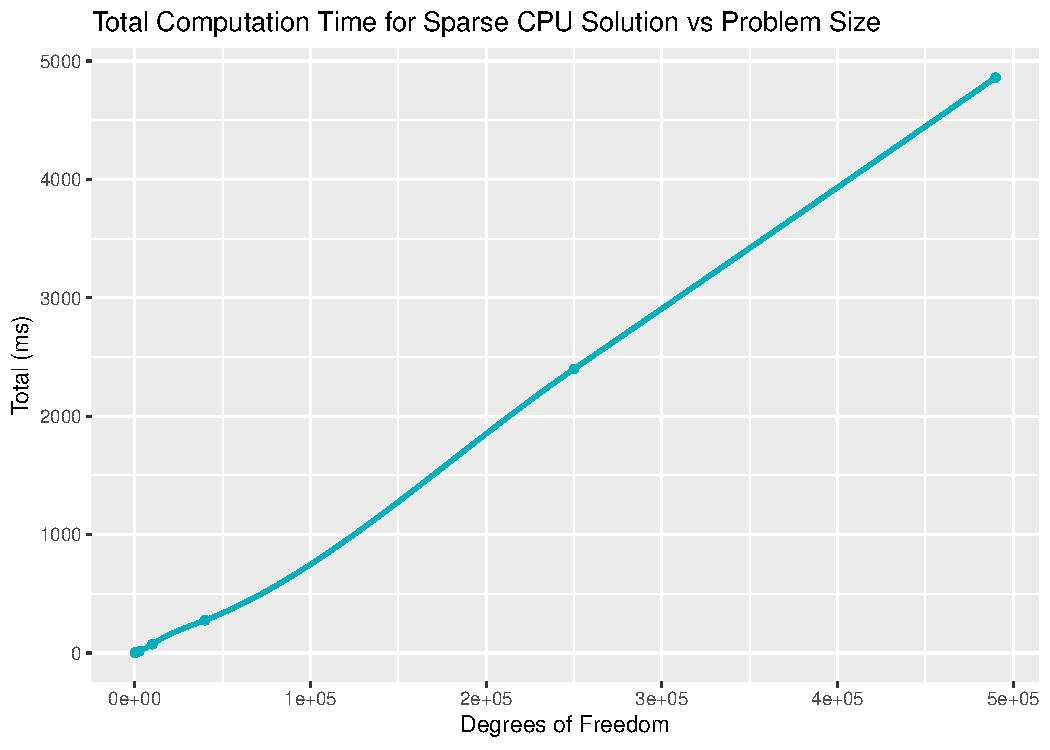
\includegraphics[width = \linewidth]{Plots/total_sparse_cpu}
		\caption{Total time taken for sparse case.}
		\label{fig:tot_sparse_cpu}
	\end{subfigure}\hfill
	\begin{subfigure}{0.48\linewidth}
		\centering
		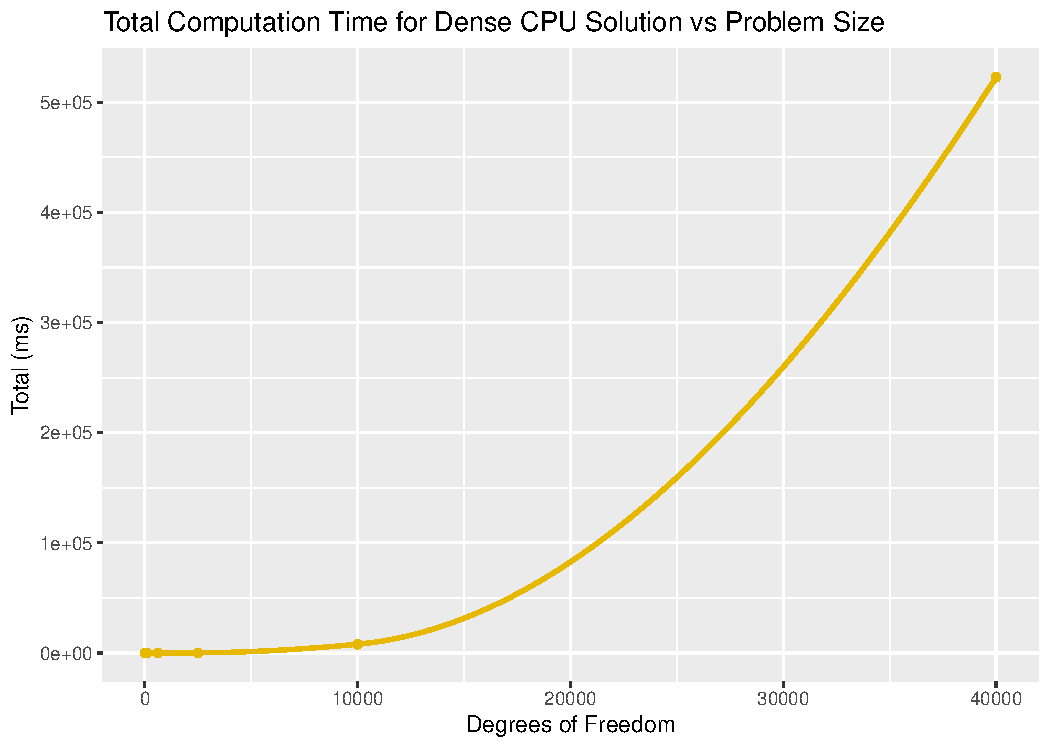
\includegraphics[width=\linewidth]{Plots/total_dense_cpu}
		\caption{Total time taken for dense case.}
		\label{fig:tot_dense_cpu}
	\end{subfigure}
	\caption{Total time taken for serial sparse and dense cases versus problem size.}
	\label{fig:tot_cpu}
\end{figure}

Figure~\ref{fig:tot_cpu} shows the total time taken in ms for the serial code to complete in both dense matrix and CSR variants. Clearly, the sparse case achieves a near linear scaling and appears to perform quite efficiently as the number of unknowns increases. The dense case on the other hand appears to have quadratic scaling, and takes orders longer time to complete as it gets larger. As mentioned in Section~\ref{sparse}, the benefit of using CSR can be huge by comparison to solving a dense system, particularly for systems as predictably sparse as the FEM. Figure~\ref{fig:cpu_tot_su} shows a logarithmic speed-up scaling of the sparse solution over the dense, reaching up to $5000\times$ faster. As it turns out, there is a couple of contributing factors here, the first being that the direct dense solvers simply do not actually scale very well in any case, and the second is that, not alone do sparse direct solvers scale better, but also, the Intel's DSS solver is a very efficient and well written piece of software compared to their dense LAPACK library. 

\begin{figure}
	\centering
	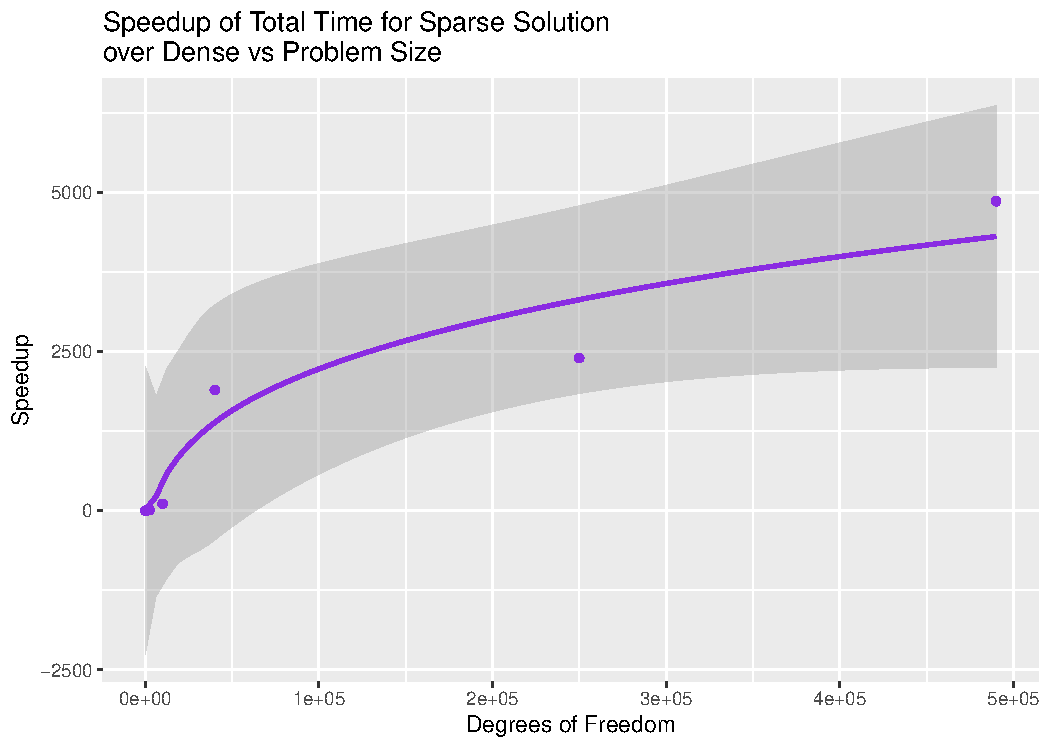
\includegraphics[width=0.48\linewidth]{Plots/total_sparse_dense_cpu_speedup_vs_n}
	\caption{Speed-up of serial sparse solution total time over dense solution versus problem size.}
	\label{fig:cpu_tot_su}
\end{figure}

\begin{figure}
	\centering
	\begin{subfigure}{0.48\linewidth}
		\centering
		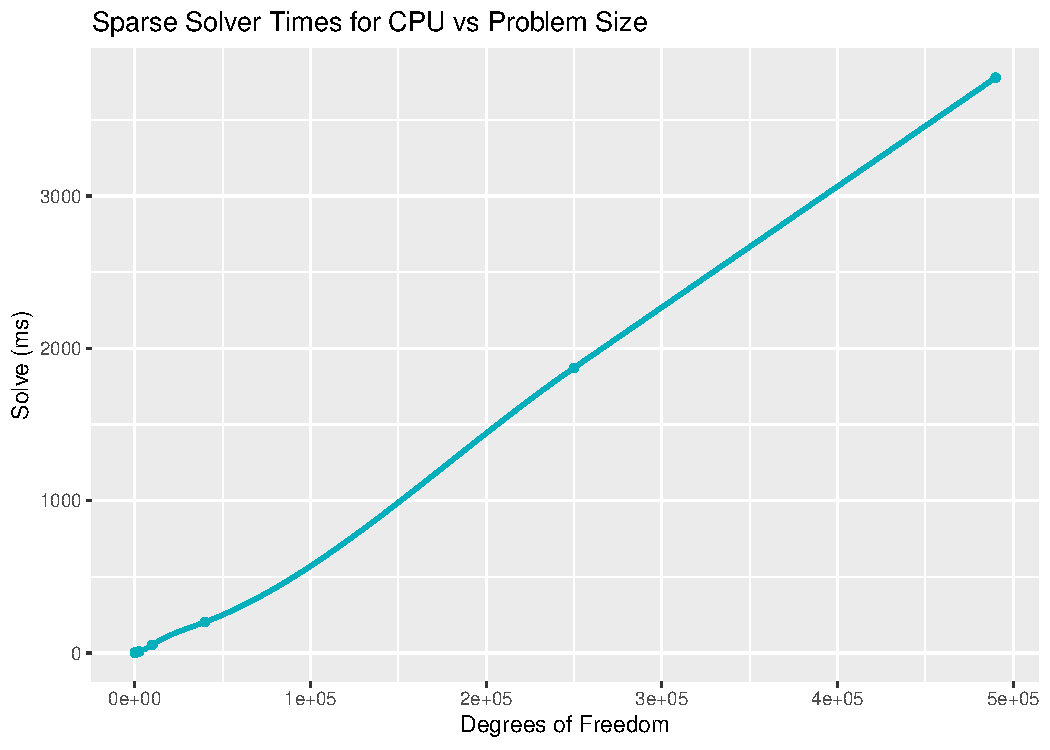
\includegraphics[width = \linewidth]{Plots/solve_sparse_cpu}
		\caption{Time taken for sparse solver.}
		\label{fig:solve_sparse_cpu}
	\end{subfigure}\hfill
	\begin{subfigure}{0.48\linewidth}
		\centering
		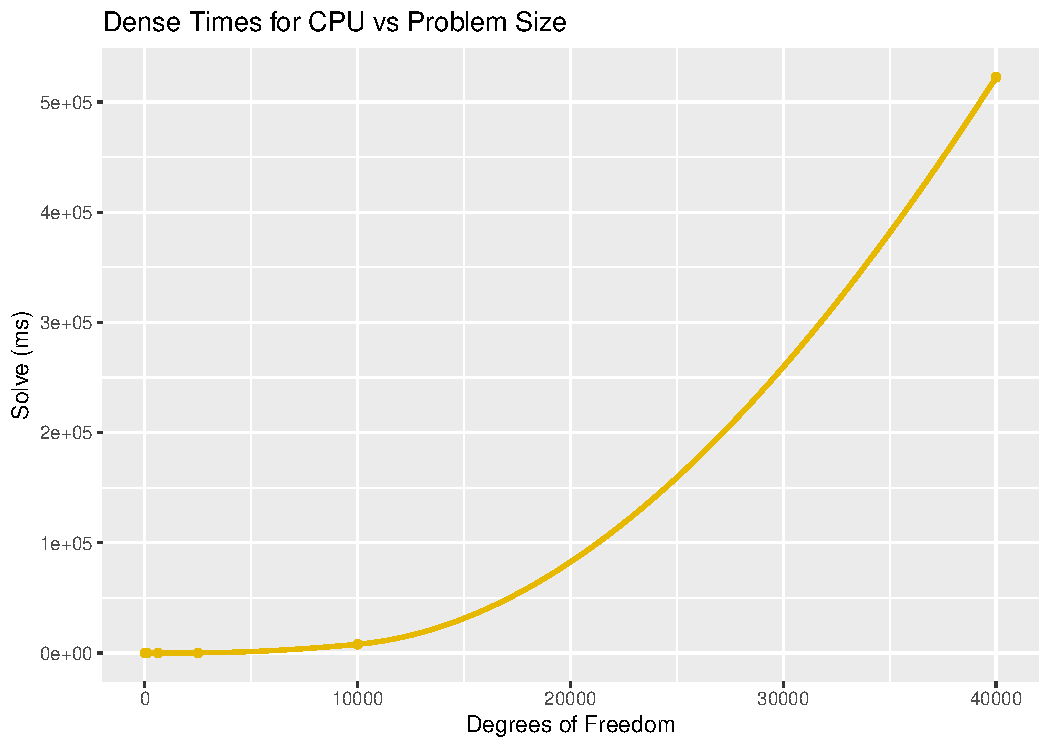
\includegraphics[width=\linewidth]{Plots/solve_dense_cpu}
		\caption{Time taken for dense solver.}
		\label{fig:solve_dense_cpu}
	\end{subfigure}
	\caption{Time taken for linear solvers in serial sparse and dense cases versus problem size.}
	\label{fig:solve_cpu}
\end{figure}

The logic behind this inference, that the solvers are what is causing the non-linear scaling, is relating to their dominance in the total computation time. Figure~\ref{fig:solve_cpu} shows the times taken for both sparse and dense solvers. Both Figures are near identical to Figure~\ref{fig:tot_cpu}, clearly demonstrating that the solvers are taking up almost all the computation time and driving the scaling pattern. Figure~\ref{fig:prop_cpu} actually illustrates far better this dominance, showing the proportion of computation time taken by the various kernels in the FEM. It also demonstrates the better scaling of the sparse solver, the proportion of which remains relatively constant as the problem size gets larger, unlike the dense solver which tends towards 100\%. The smallest problem sizes were removed from both charts as the timing was too small to actually get an accurate representation.

\begin{figure}
	\centering
	\begin{subfigure}{0.48\linewidth}
		\centering
		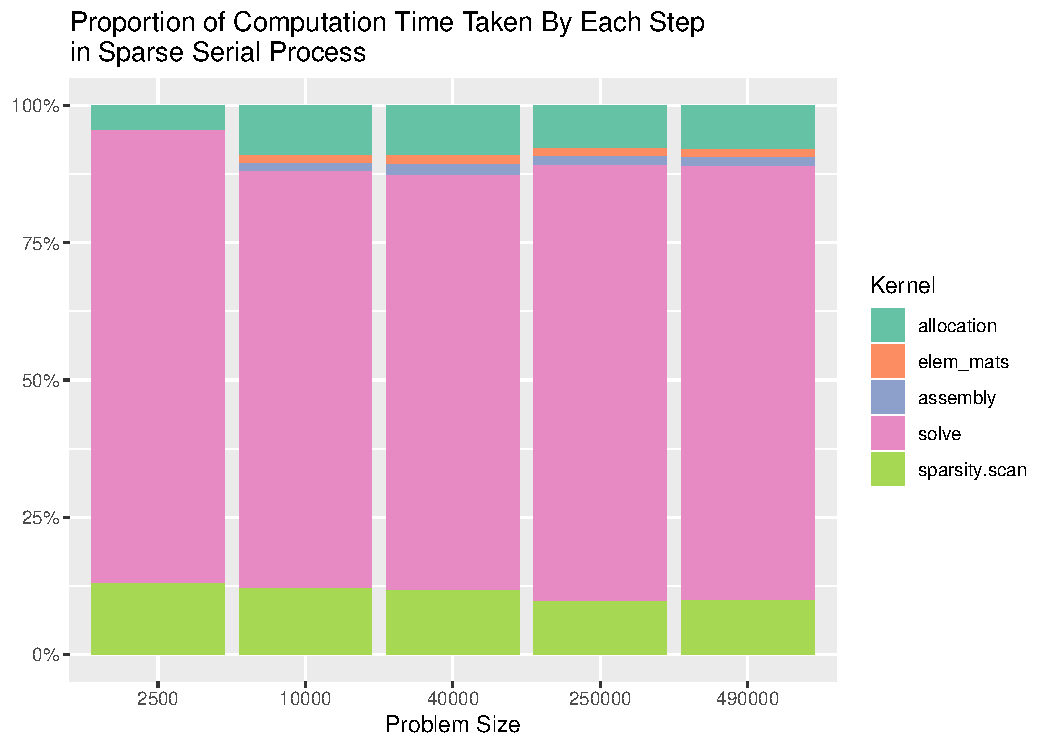
\includegraphics[width = \linewidth]{Plots/prop_sparse}
		\caption{Proportion of time taken for each kernel in sparse solution.}
		\label{fig:prop_sparse}
	\end{subfigure}\hfill
	\begin{subfigure}{0.48\linewidth}
		\centering
		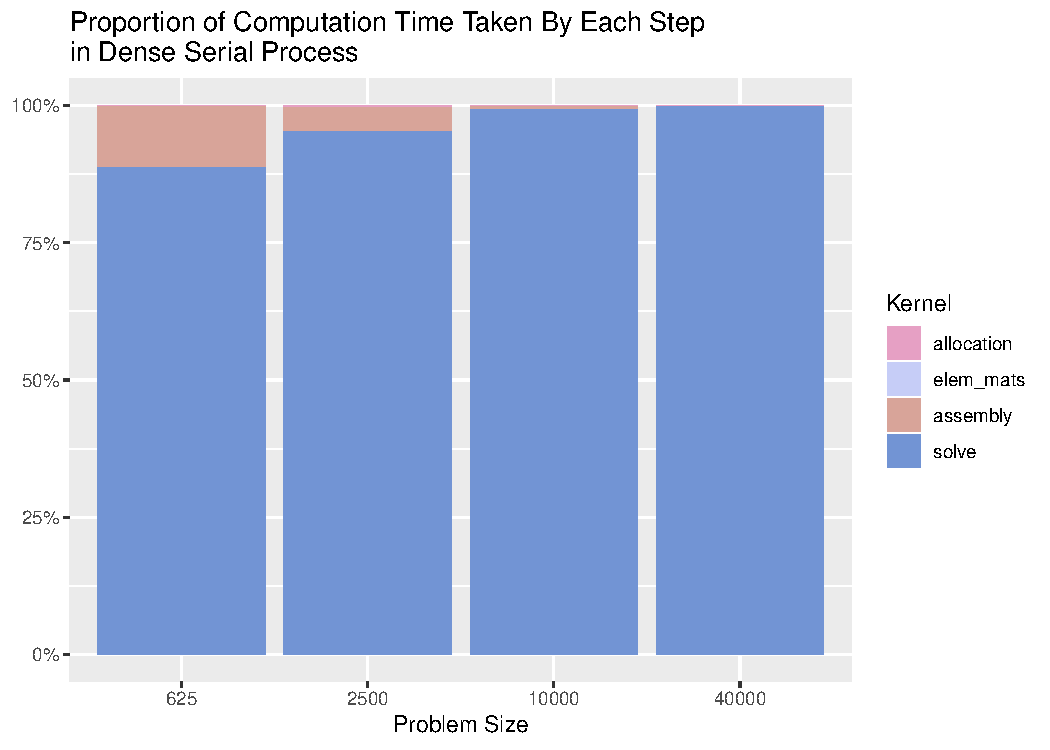
\includegraphics[width=\linewidth]{Plots/prop_dense}
		\caption{Proportion of time taken for each kernel in dense solution.}
		\label{fig:prop_dense_cpu}
	\end{subfigure}
	\caption{Proportion of computation time taken per kernel for sparse and dense CPU cases.}
	\label{fig:prop_cpu}
\end{figure}

In terms of the profiling and performance of the other kernels involved in the process, Figure~\ref{fig:kerns} shows the timings taken for the generation of the element matrices, assembling both CSR and dense global stiffness matrices and the sparsity scan performed a priori. Most of the Figures show a linear scaling, barring Figure~\ref{fig:assem_dense_n}, showing a slight quadratic scaling - to be expected given the quadratic scaling in matrix size.

\begin{figure}
	\centering
	\begin{subfigure}{0.48\linewidth}
		\centering
		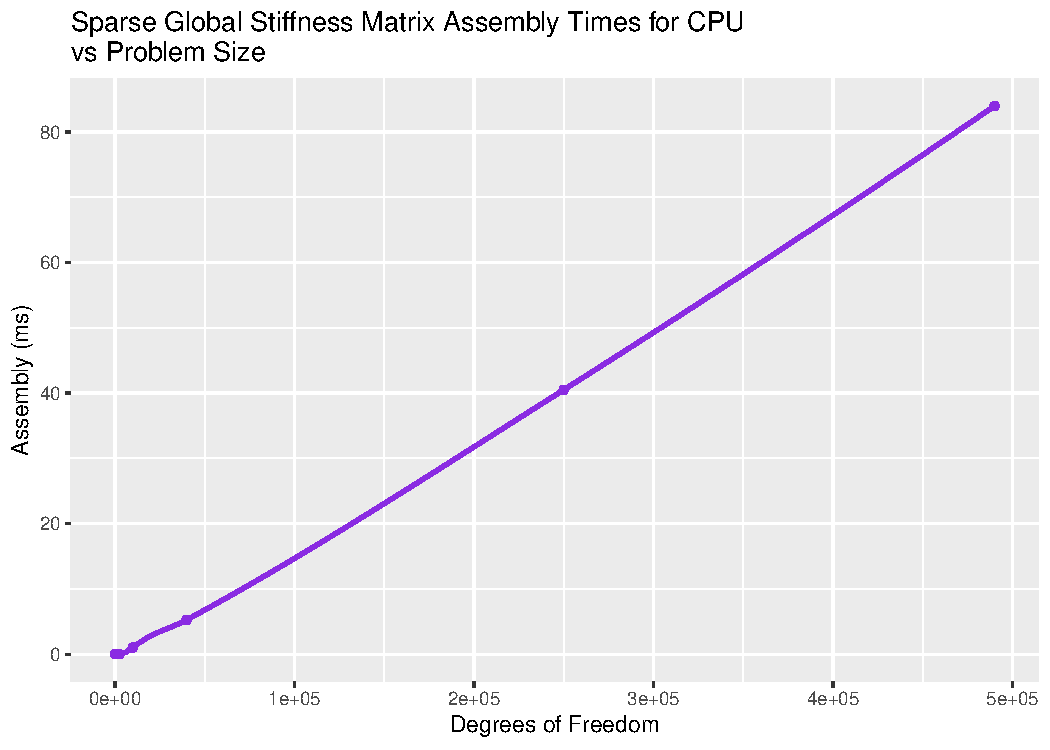
\includegraphics[width = \linewidth]{Plots/assembly_sparse_cpu}
		\caption{Time taken for assembly of CSR global stiffness matrix.}
		\label{fig:assem_sparse}
	\end{subfigure}\hfill
	\begin{subfigure}{0.48\linewidth}
		\centering
		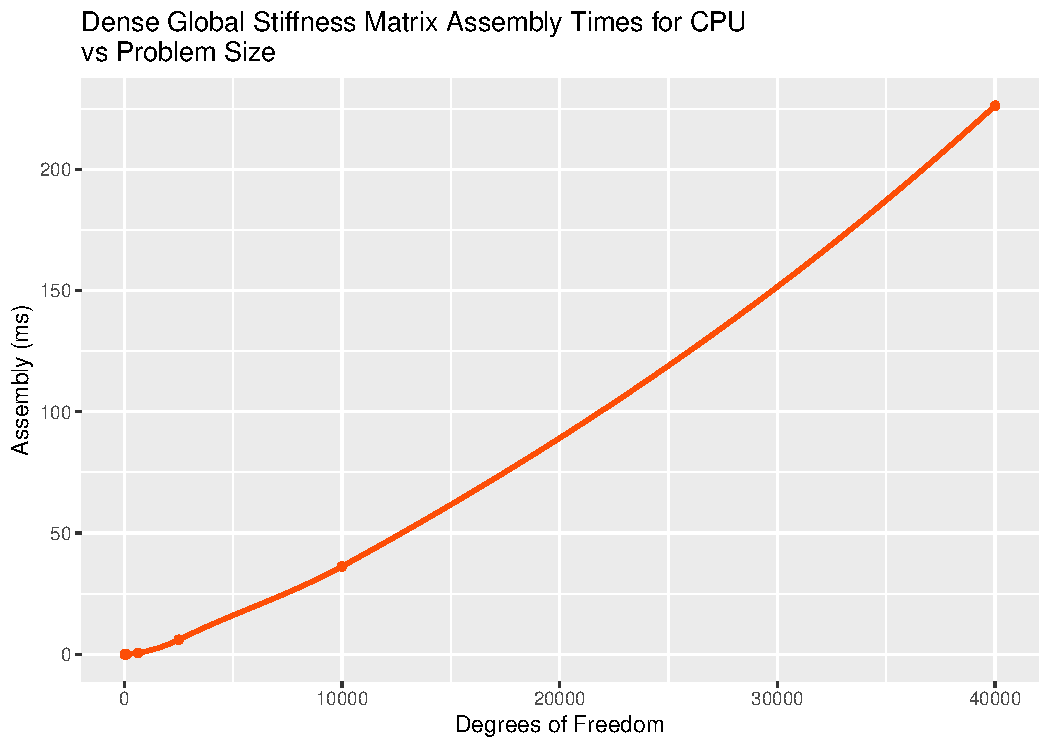
\includegraphics[width=\linewidth]{Plots/assembly_dense_cpu}
		\caption{Time taken for assembly of dense global stiffness matrix.}
		\label{fig:assem_dense}
	\end{subfigure}\\
	\begin{subfigure}{0.48\linewidth}
		\centering
		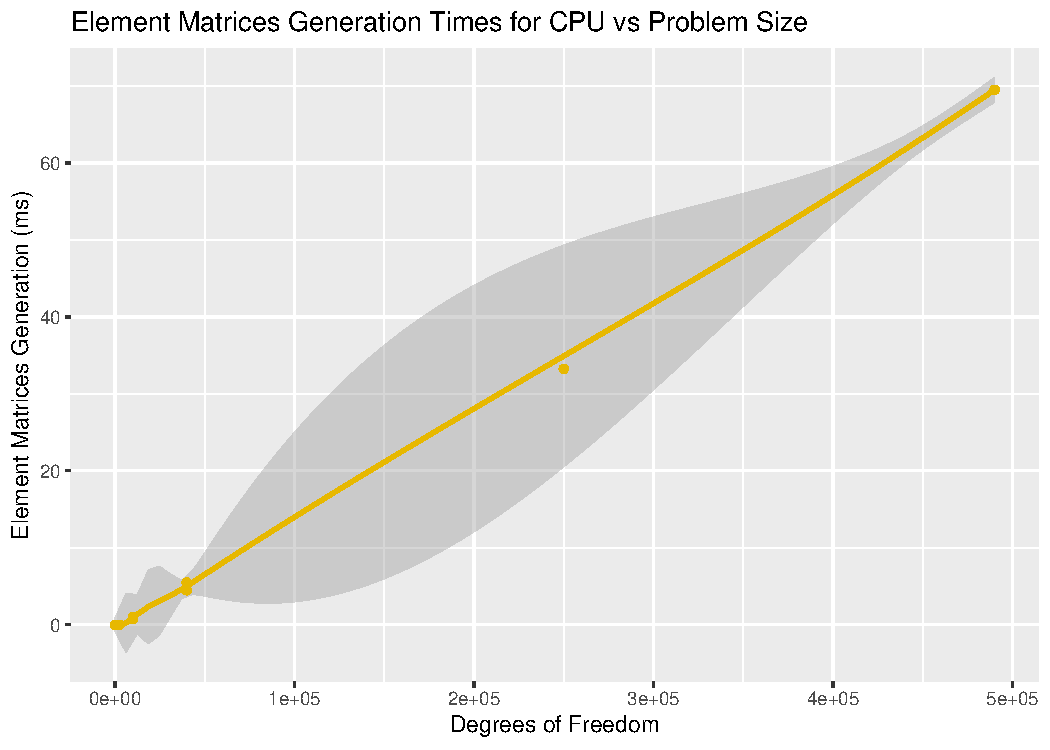
\includegraphics[width=\linewidth]{Plots/elem_mats_cpu}
		\caption{Time taken for generation of element matrices.}
		\label{fig:elems_sparse}
	\end{subfigure}\hfill
	\begin{subfigure}{0.48\linewidth}
		\centering
		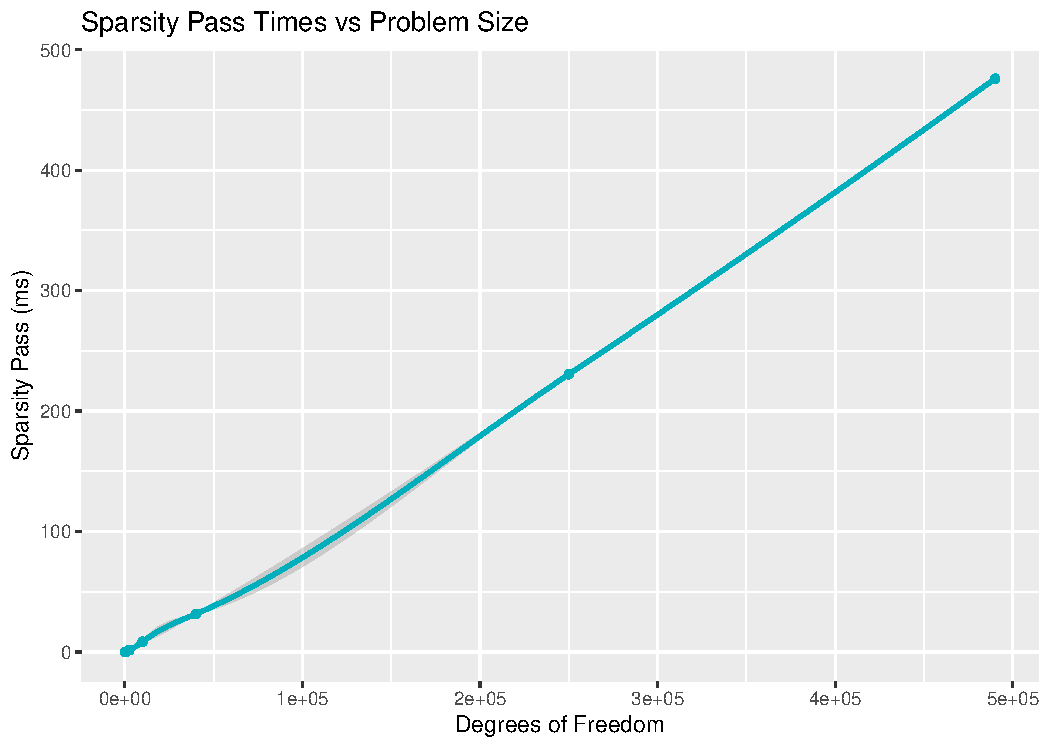
\includegraphics[width=\linewidth]{Plots/sparsity_pass_cpu}
		\caption{Time taken to perform sparsity pass.}
		\label{fig:sparsity_scan}
	\end{subfigure}
	\caption{Timings taken versus problem size for various kernels involved in CPU FEM method.}
	\label{fig:kerns}
\end{figure}

\subsubsection{Results}

Figure~\ref{fig:results} shows a 3D plot of the resulting solution to the PDE achieved by the serial implementation for a $200\times 200$ case.

\begin{figure}
	\centering
	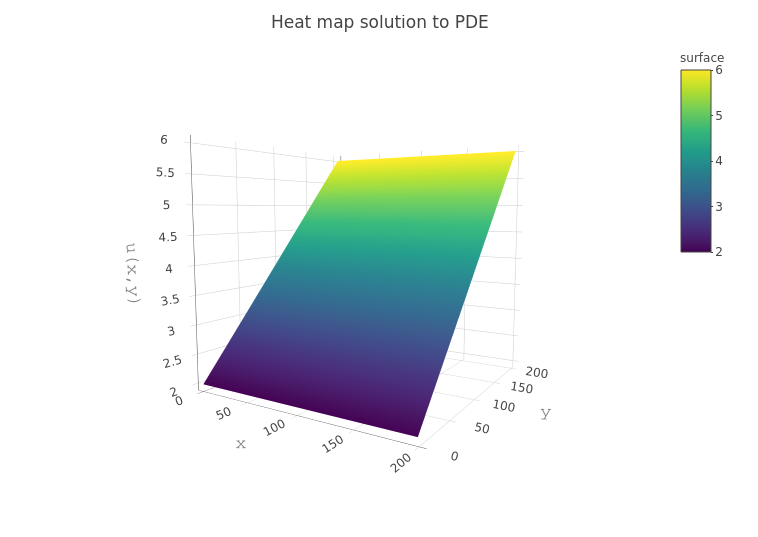
\includegraphics[width = 0.8\linewidth]{Plots/3d_soln}
	\caption{Plot of solution to Laplace equation posed in Section~\ref{problem} generated by serial implementation.}
	\label{fig:results}
\end{figure}
\section{GPU Performance}

\subsection{Standard FEM}

The standard FEM GPU approach achieved some varying times, depending largely on whether or not sparse or dense solvers were used. The generation of the element matrices, and assembly of the stiffness matrices reached some quite substantial speed-ups. However, as is detailed in this section, these kernel timings were dominated by the far more computationally expensive linear solvers.

\subsubsection{Total Timings}

\begin{figure}
	\centering
	\begin{subfigure}{0.48\linewidth}
		\centering
		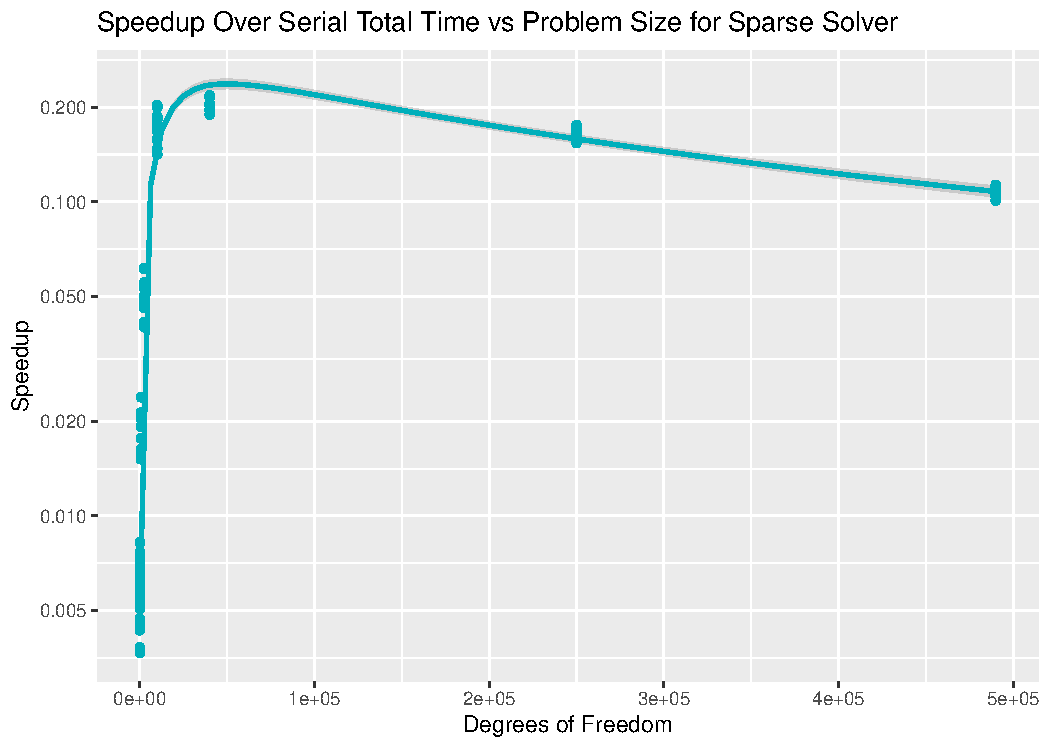
\includegraphics[width = \linewidth]{Plots/total_sparse_cpu_speedup_vs_n}
		\caption{Total time speed-up over sparse serial solution.}
		\label{fig:tot_sparse}
	\end{subfigure}\hfill
	\begin{subfigure}{0.48\linewidth}
		\centering
		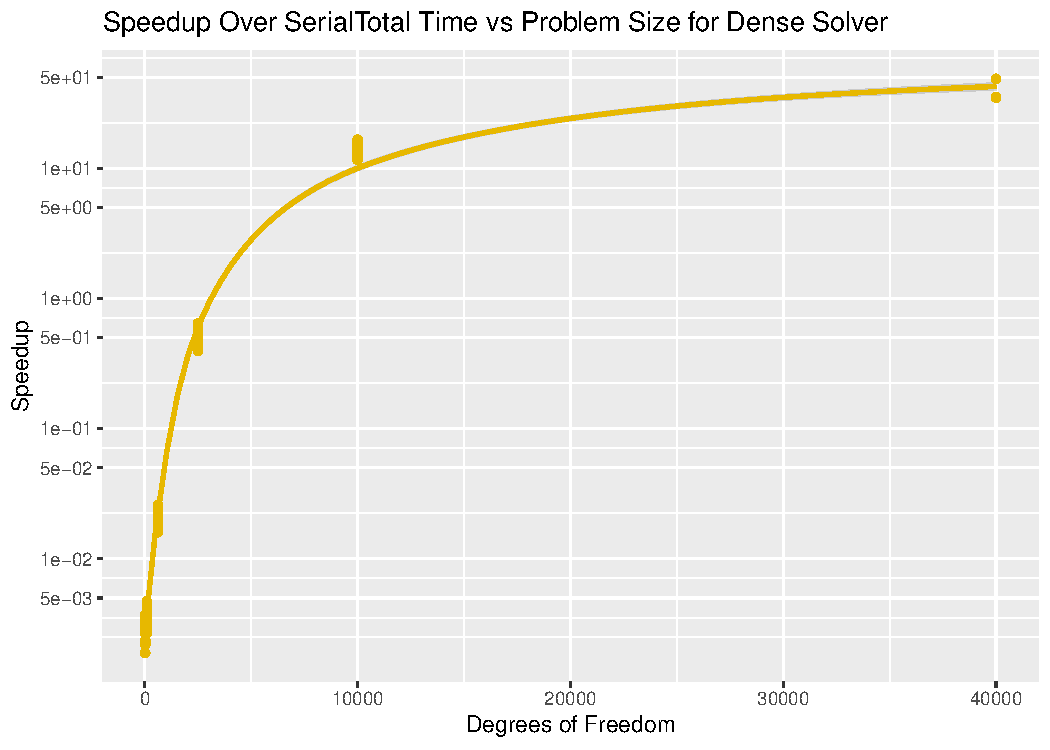
\includegraphics[width=\linewidth]{Plots/total_dense_cpu_speedup_vs_n}
		\caption{Total time speed-up over dense serial solution.}
		\label{fig:tot_dense}
	\end{subfigure}\\
	\begin{subfigure}{0.48\linewidth}
		\centering
		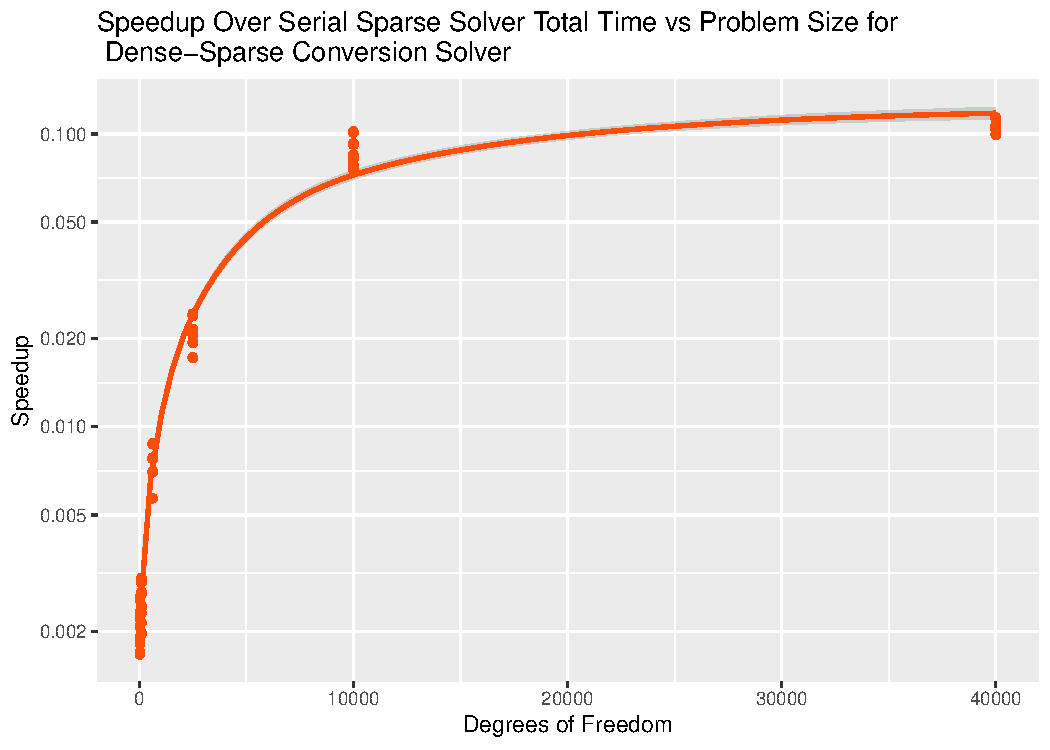
\includegraphics[width=\linewidth]{Plots/total_dnsspr_cpu_sparse_speedup_vs_n}
		\caption{Total time speed-up dense-sparse conversion method over sparse serial solution.}
		\label{fig:tot_dnsspr_sparse}
	\end{subfigure}\hfill
	\begin{subfigure}{0.48\linewidth}
		\centering
		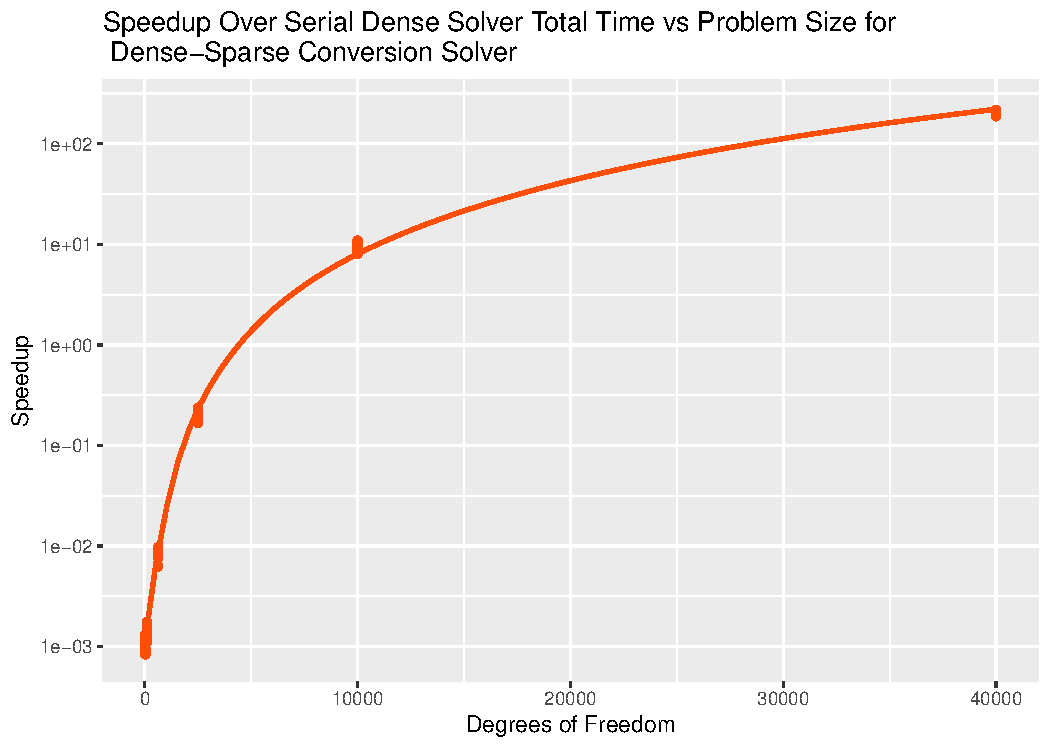
\includegraphics[width=\linewidth]{Plots/total_dnsspr_cpu_dense_speedup_vs_n}
		\caption{Total time speed-up dense-sparse conversion method over dense serial solution.}
		\label{fig:tot_dnsspr_dense}
	\end{subfigure}
	\caption{Speed-ups of total GPU times over serial code vs. problem size for sparse, dense and dense-sparse conversion solutions.}
	\label{fig:tot}
\end{figure}

Figure~\ref{fig:tot} illustrates the speed-ups of the total timings taken to complete the FEM for the various solver approaches against problem size. Looking initially at the sparse or CSR variant, Figure~\ref{fig:tot_sparse} shows the speed-up over the sparse serial case. Clearly it does not actually achieve a speed-up at all, but is in fact slower for all problem sizes. It does demonstrate and initial spike, but this can be written down to simply a factor of GPU programming. Often, for small problem sizes, there are initial costs of transferring data from host to device, allocating memory on the device's DRAM and even just the card needing to "warm-up" - for lack of a better term.  For small problem sizes, this cost is proportionally much larger, and clearly as the number of unknowns grows, this factors in less. There is also, naturally, much less parallelisation achievable at smaller problem sizes than larger ones. Thus, this spike is natural and to be expected and not really a result to be concerned about. What is more concerning was the lack of positive scaling. As it turns out, the total time is quite substantially dominated by the cuSOLVER sparse direct solver, which happens to not perform anywhere near as optimally as Intel's DSS, and even sees a decreasing scaling as problem size gets larger - though there is little can be done about that unfortunately.

The dense solver, from a glance at Figure~\ref{fig:tot_dense}, demonstrates far more promising results. There is a clear logarithmic scaling present in the graph. However, again from the offset with small problem sizes, parallelising the problem is not worth it, and results in slower times. However, evidently, this improves quite rapidly and as the degrees of freedom approach 40,000, the solver outperforms the serial code by a speed-up of around $50\times$. Again here, there is a substantial proportion of the computation time taken up by the linear solver which is shown later.

The dense-sparse conversion was compared to both the serial CSR solver and the serial dense solver in Figures~\ref{fig:tot_dnsspr_sparse}~\ref{fig:tot_dnsspr_dense}, since it sits somewhere in between both, having a dense assembly and sparse solver. Given the proportion of computation time is considerable, it is to be expected that the dense-sparse solver performs poorly also by comparison to Intel's DSS - which it indeed does. The scaling has the same spike as the sparse-sparse comparison, though it is not immediately obvious due to memory limitations not permitting allocation of  larger problem sizes - which the pure CSR solver had the benefit of avoiding to a larger extent. This solver drastically outperforms the purely dense serial solution, achieving large speed-ups of up to $100\times$.

Figure~\ref{fig:tot_b} shows the speed-ups seen over the CPU code for sparse and dense solutions versus the choice of block size input from the command line. Without yet going into the details of the linear solvers computational dominance, in both cases, the stability in timings with variation of block size should tell enough that, the purpose-written code has little actual impact on the resulting final timings. A benefit of the linear solvers is that they are optimised such that the best choice of block size to reduce warp divergence and maximise shared memory usage is selected for the user. Thus, meaning the choice of block size, should have not much impact - shown very much so in Figure~\ref{fig:tot_b}. Rather interestingly though, it does show the nice scaling with problem size for the dense case in Figure~\ref{fig:tot_dense_b} and the decreasing scaling for the sparse case in Figure~\ref{fig:tot_sparse_b}, where 40,000 degrees of freedom achieves more speed-up than 490,000.

\begin{figure}
	\centering
	\begin{subfigure}{0.48\linewidth}
		\centering
		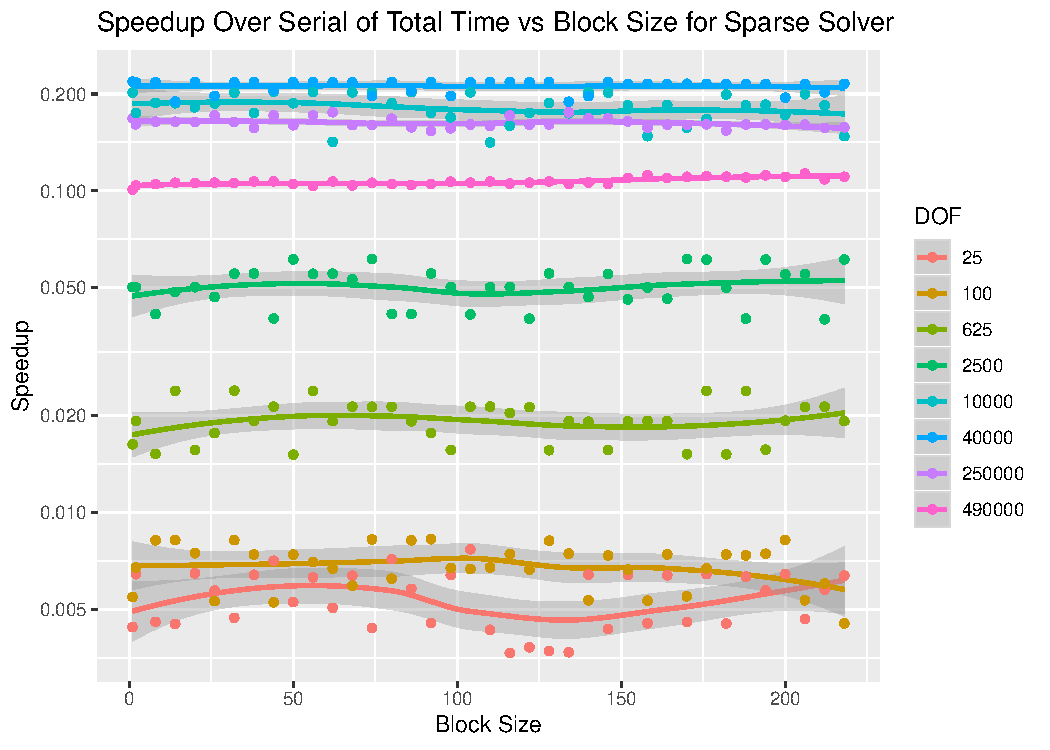
\includegraphics[width = \linewidth]{Plots/total_sparse_cpu_speedup_vs_b}
		\caption{Total time speed-up over sparse serial solution.}
		\label{fig:tot_sparse_b}
	\end{subfigure}\hfill
	\begin{subfigure}{0.48\linewidth}
		\centering
		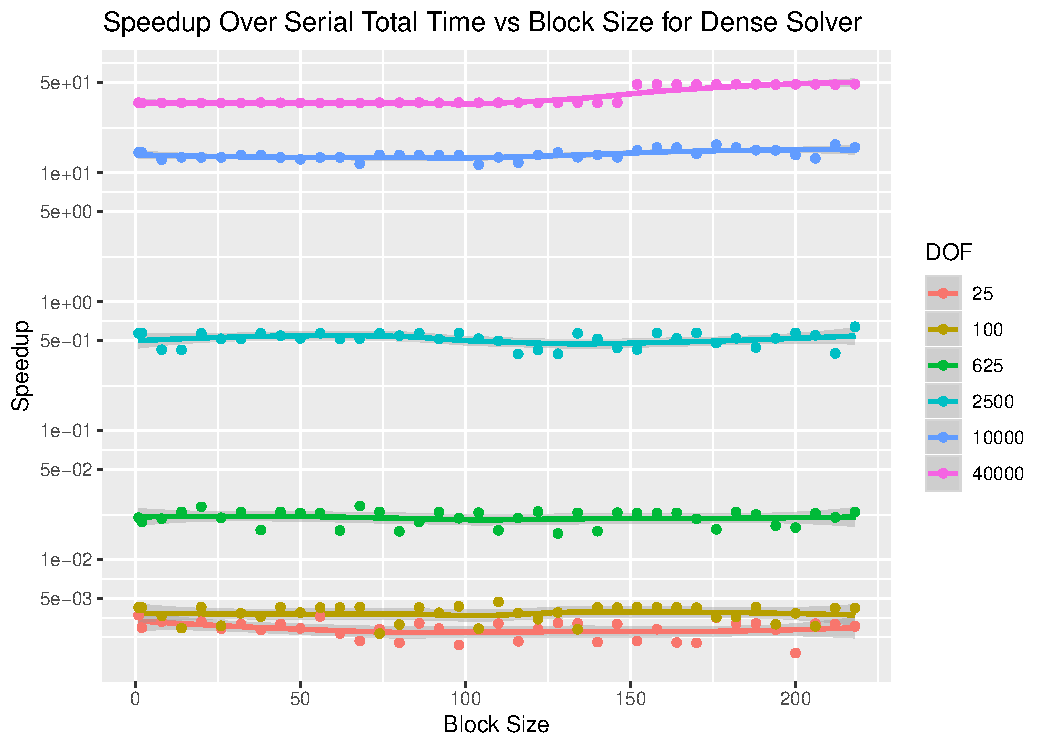
\includegraphics[width=\linewidth]{Plots/total_dense_cpu_speedup_vs_b}
		\caption{Total time speed-up over dense serial solution.}
		\label{fig:tot_dense_b}
	\end{subfigure}
	\caption{Speed-ups of total GPU times over serial code versus block size, for sparse and dense solutions.}
	\label{fig:tot_b}
\end{figure}

\subsubsection{Linear Solvers}

\begin{figure}
	\centering
	\begin{subfigure}{0.48\linewidth}
		\centering
		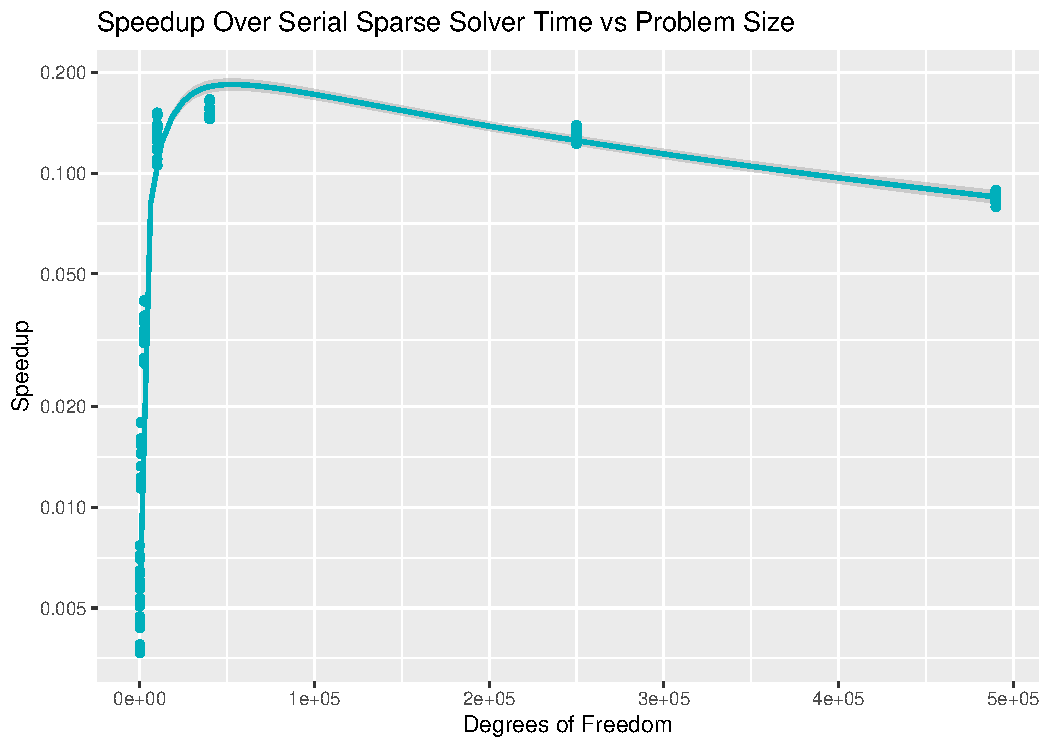
\includegraphics[width = \linewidth]{Plots/solve_sparse_cpu_speedup_vs_n}
		\caption{Sparse solver speed-up over Intel's MKL DSS.}
		\label{fig:sparse_solver}
	\end{subfigure}\hfill
	\begin{subfigure}{0.48\linewidth}
		\centering
		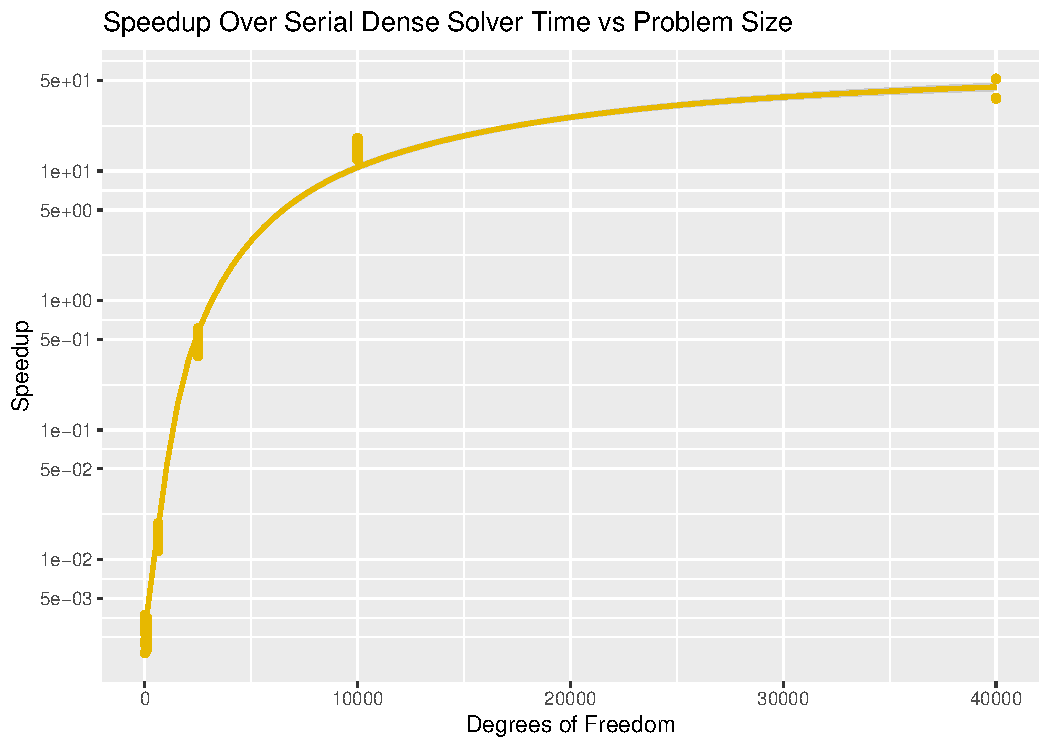
\includegraphics[width=\linewidth]{Plots/solve_dense_cpu_speedup_vs_n}
		\caption{Dense solver speed-up over Intel's MKL LAPACKE.}
		\label{fig:dense_solver}
	\end{subfigure}
	\caption{Speed-ups of cuSOLVER's solver times over Intel's MKL versus problem size, for sparse and dense solutions.}
	\label{fig:solvers}
\end{figure}
Looking at the actual performance of the linear solvers themselves, Figures~\ref{fig:sparse_solver},~\ref{fig:dense_solver} almost identically replicate the results seen in Figures~\ref{fig:tot_sparse},~\ref{fig:tot_dense} - just more illustrating how dominant these are towards the total time taken. In Figure~\ref{fig:sparse_prop}, this can be seen from screen-shots taken from Nvidia's Visual Profiler where the massive chunk of computation time taken by these solvers, for a relatively small problem size of 2,500, compared to the rest the FEM process is shown - the kernel written for this report takes 0.4\%. It isn't that these wholly perform poorly, more-so that Intel's DSS solve for CSR linear systems is optimised to very impressive levels, and simply outperforms Nvidia's cuSOLVER and cuSPARSE solutions. The dense solver on the other hand actually performs quite well compared to Intel's MKL library. It was not the premise of this paper to improve on existing direct linear solvers so this is simply a result that needs to be taken with a pinch of salt.

\begin{figure}
	\centering
	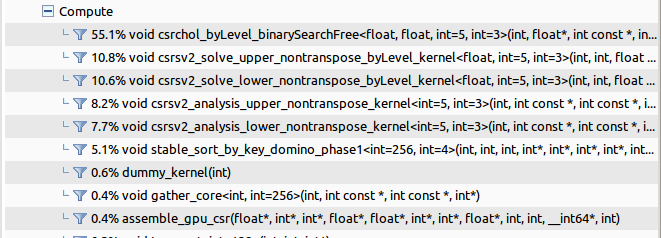
\includegraphics[width = 0.7\linewidth]{Figures/sparse_prop_50}
	\caption{Proportion of computation time taken by various kernels involved shown in Nvidia's Visual Profiler for a problem size of 2,500 unknowns for sparse GPU method.}
	\label{fig:sparse_prop}
\end{figure}

While it may seem that Nvidia's CSR solver is actually a poorly written and poorly performing piece of software, and one would be better off using the dense solver - this is certainly not the case, it just happens to not be as optimised as Intel's. Figure~\ref{fig:gpu_solve} illustrates the speed-ups of the sparse solver over the dense solver as problem size increases. Notably, it gets up to around $10\times$ speed-up and is, in fact, a better performing solution than assembling a dense system and solving. This is the benefits mentioned in Section~\ref{sparse} visibly in action.

\begin{figure}
	\centering
	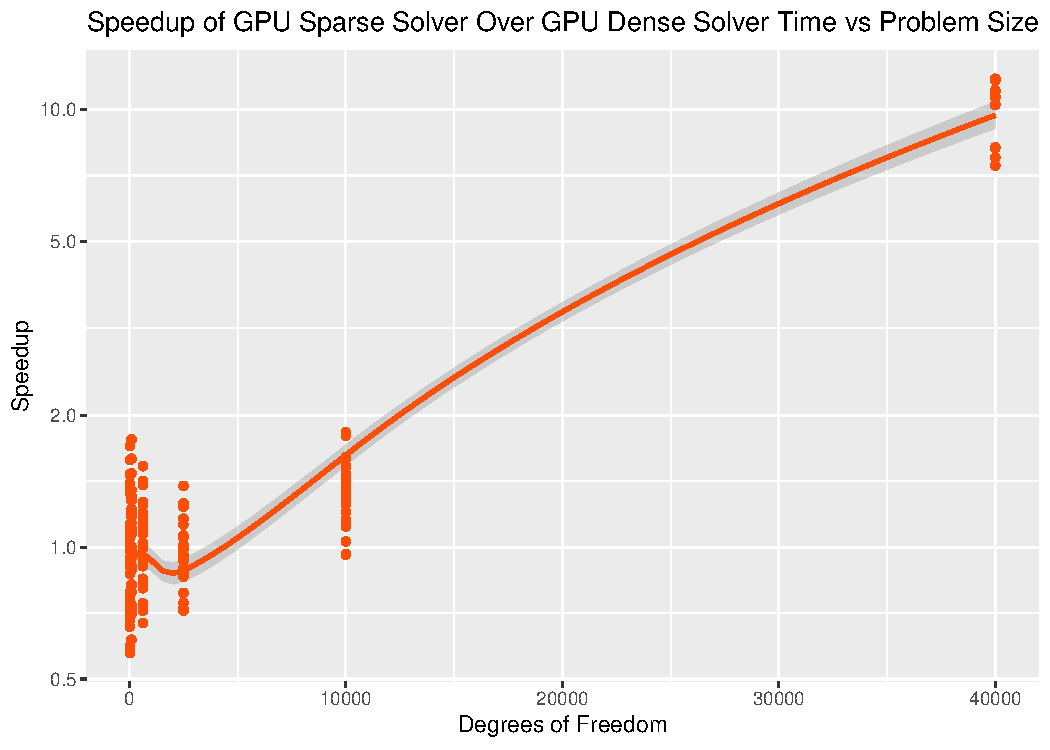
\includegraphics[width = 0.48\linewidth]{Plots/solve_gpus_speedup_vs_n}
	\caption{Speed-ups of cuSOLVER's sparse linear solver over cuSOLVER's dense solver against problem size.}
	\label{fig:gpu_solve}
\end{figure}

\subsubsection{Allocations \& Transfers}

\begin{figure}
	\centering
	\begin{subfigure}{0.48\linewidth}
		\centering
		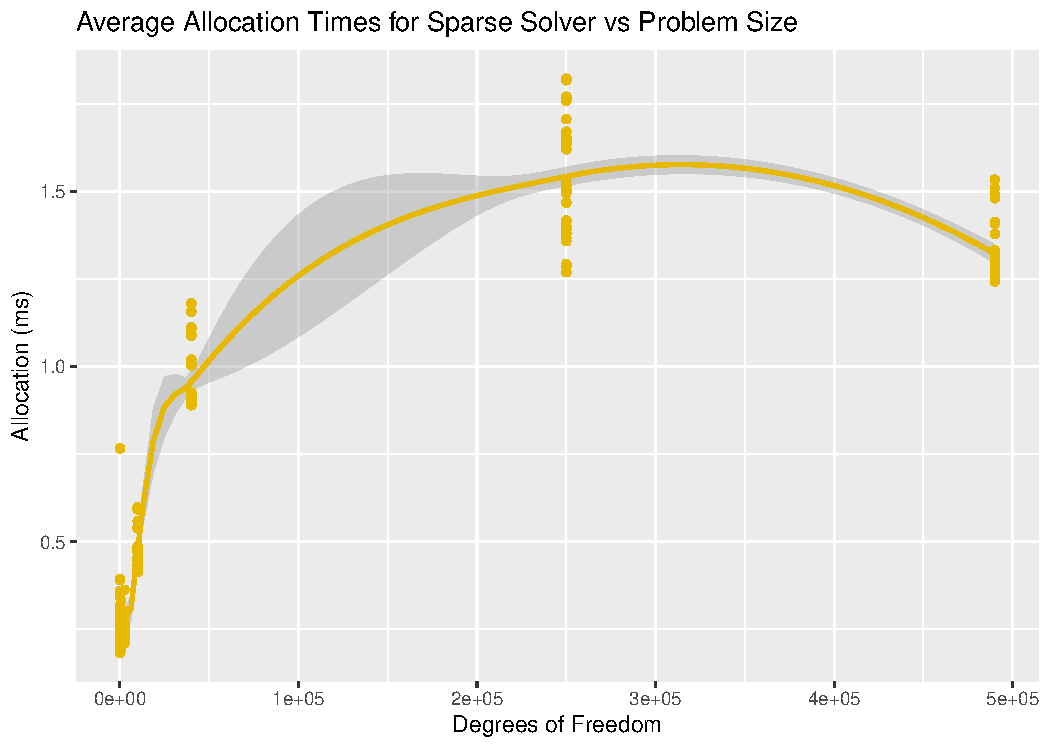
\includegraphics[width = \linewidth]{Plots/alloc_sparse_vs_n}
		\caption{Allocation time taken for sparse case.}
		\label{fig:alloc_sparse}
	\end{subfigure}\hfill
	\begin{subfigure}{0.48\linewidth}
		\centering
		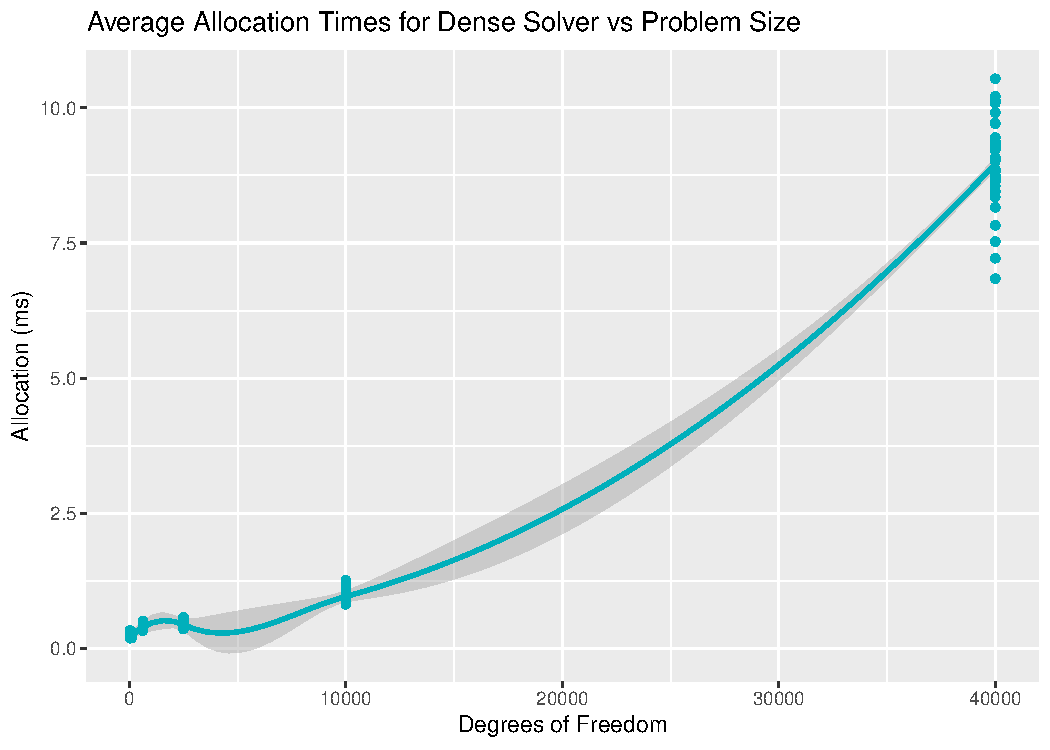
\includegraphics[width=\linewidth]{Plots/alloc_dense_vs_n}
		\caption{Allocation time taken for dense case.}
		\label{fig:alloc_dense}
	\end{subfigure}
	\caption{Total allocation time taken for both dense and CSR GPU approaches.}
	\label{fig:alloc}
\end{figure}
Figure~\ref{fig:alloc} shows the total allocation times for both sparse and dense cases. The dense case seen in Figure~\ref{fig:alloc_dense}, is not expected to have a linear scaling but more so a polynomial scaling. It illustrates a 2\textsuperscript{nd} order polynomial scaling, this is to be expected since, excluding the mesh, the dominant array needing to be allocated is of size $\texttt{order}\times\texttt{order}$. The sparse case in Figure~\ref{fig:alloc_sparse}, on the other hand, is harder to predict the scaling of. This is due to the fact that as the matrix gets larger, the number of non-zeros present in the matrix will be totally dependent on the both the shape of the mesh, and the degrees of freedom chosen for the basis functions - be it P1 or P2 et cetera. The timing does appear to decrease, though the inclination here is that this it is due to variance and the small sample size of five per data point - in this case five runs per block size and problem size. Figure~\ref{fig:alloc_su} shows the speed-up seen in performing the sparse case over the dense. Since both variants allocate the five arrays needed for the mesh as well as the stiffness matrix, naturally the expected, and observed, result here is sparse speed-up over dense.
\begin{figure}
	\centering
	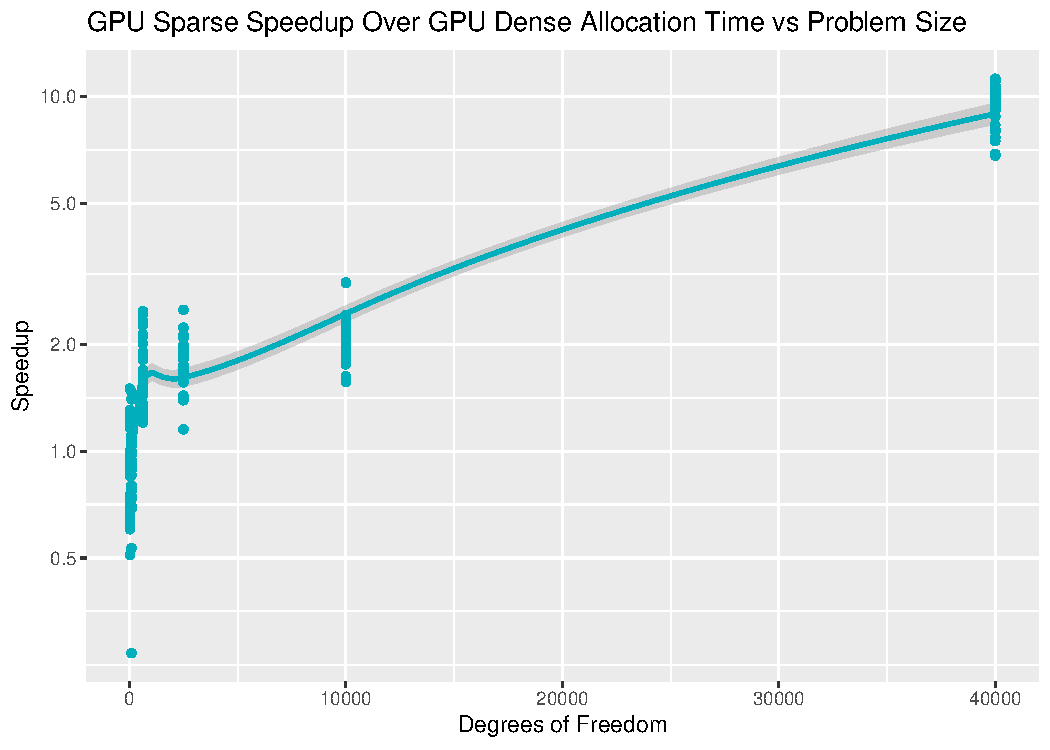
\includegraphics[width=0.48\linewidth]{Plots/alloc_sparse_dense_speedup_vs_n}
	\caption{Speed-up of allocation time taken for sparse case over dense versus problem size}
	\label{fig:alloc_su}
\end{figure}

\begin{figure}
	\centering
	\begin{subfigure}{0.48\linewidth}
		\centering
		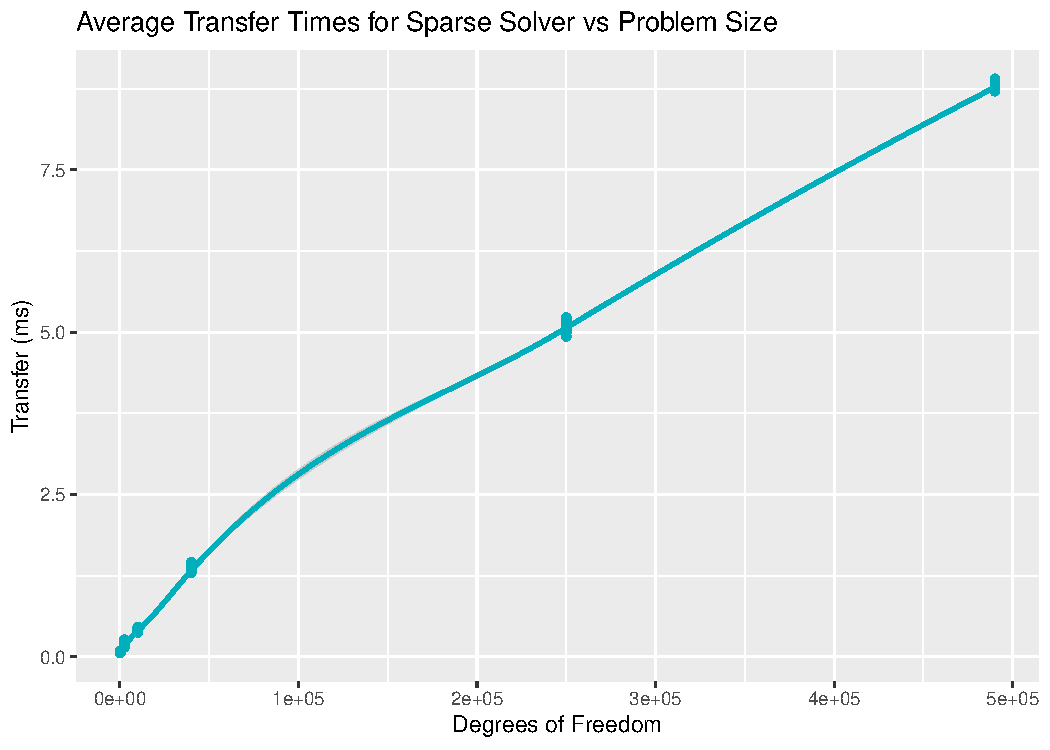
\includegraphics[width = \linewidth]{Plots/transf_sparse_vs_n}
		\caption{Transfer time taken for sparse case.}
		\label{fig:transf_sparse}
	\end{subfigure}\hfill
	\begin{subfigure}{0.48\linewidth}
		\centering
		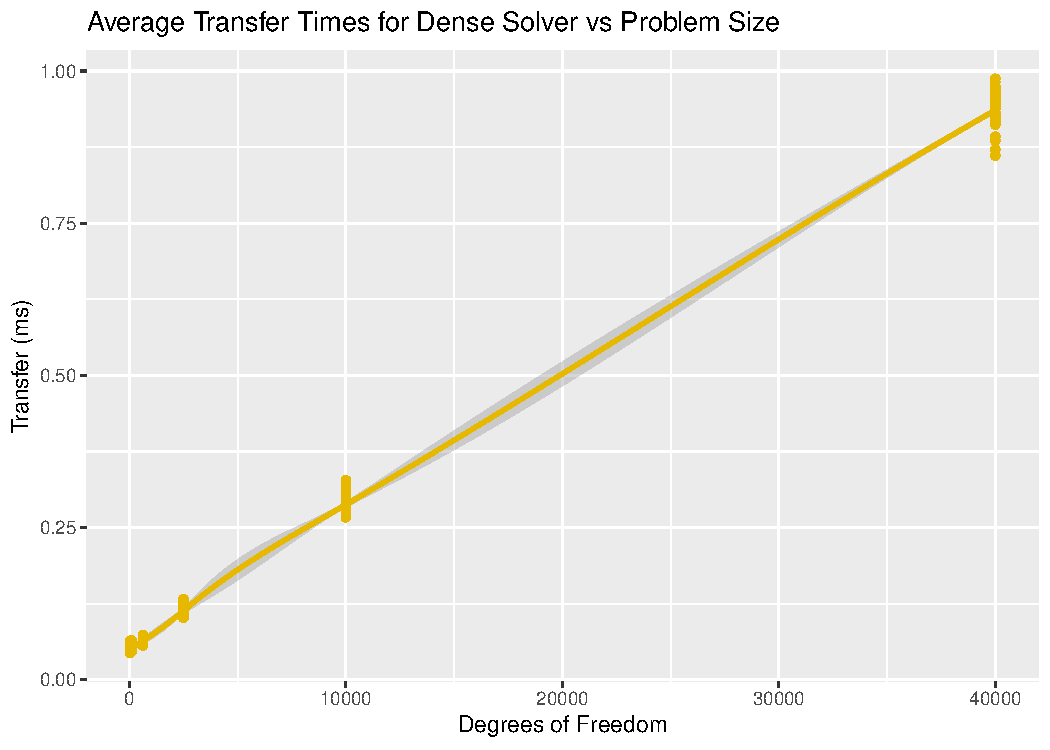
\includegraphics[width=\linewidth]{Plots/transf_dense_vs_n}
		\caption{Transfer time taken for dense case.}
		\label{fig:transf_dense}
	\end{subfigure}
	\caption{Total transfer time taken for both dense and CSR approaches.}
	\label{fig:transf}
\end{figure}

Unlike in the allocation case, the sparse timings can be a bit more predictable. For allocating, all three of the arrays for the stiffness matrix have to be allocated, as well as the array for the stress vector. For the transfer, the mesh of course, as in allocation, needs to be transferred, and solution vector or former stress vector, but only two of the three CSR arrays. This should give rise to a much more linear scaling, as demonstrated in Figure~\ref{fig:transf_sparse}. It is not a perfect linear scaling, nor should it be, but the reduced effect of the irregular scaling of the CSR matrix is definitely evident. The dense case on the other hand, only transfers the mesh and the stiffness matrix, all of which scale in size linearly and thus, as is seen in Figure~\ref{fig:transf_dense}, observe a nice linear scaling. Figure~\ref{fig:transf_su} shows the speed-up seen in the sparse case over the dense. In this case, as would be entirely presumed, the dense case takes about 70\% of the time. Of course this would be expected given there is no sparsity pattern to transfer from the host.

\begin{figure}
	\centering
	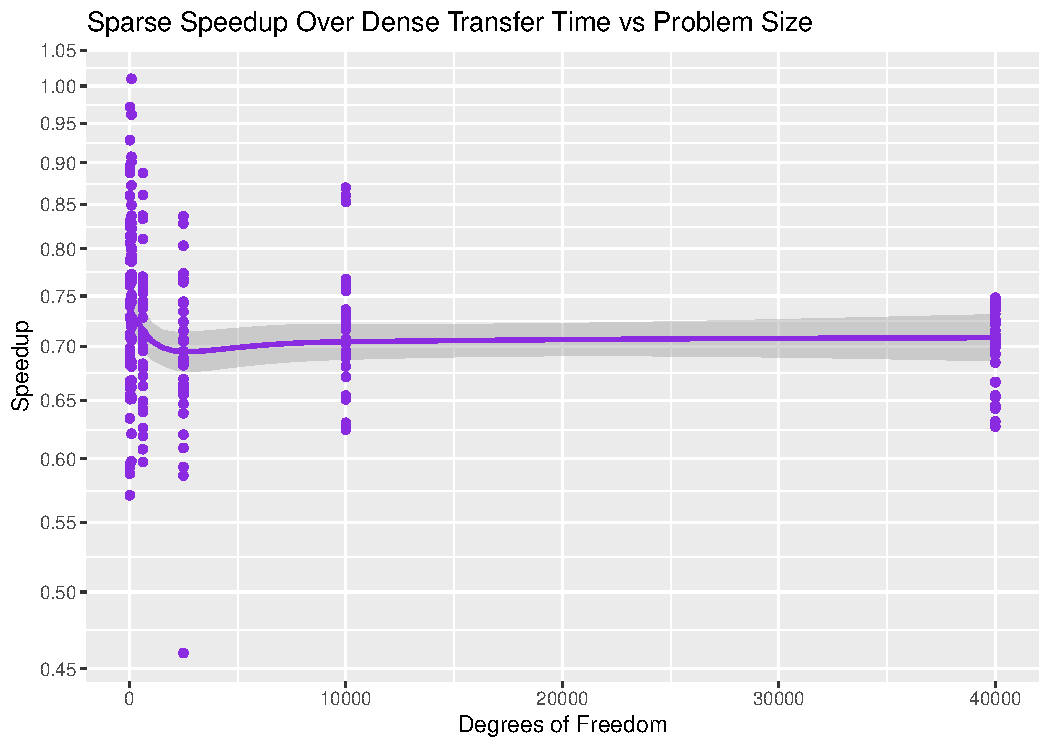
\includegraphics[width = 0.48\linewidth]{Plots/transf_sparse_dense_speedup_vs_n}
	\caption{Speed-up of transfer time for sparse case over dense case versus problem size.}
	\label{fig:transf_su}
\end{figure}

\subsubsection{Generation of Element Matrices \& Vectors}

\begin{figure}
	\centering
	\begin{subfigure}{0.48\linewidth}
		\centering
		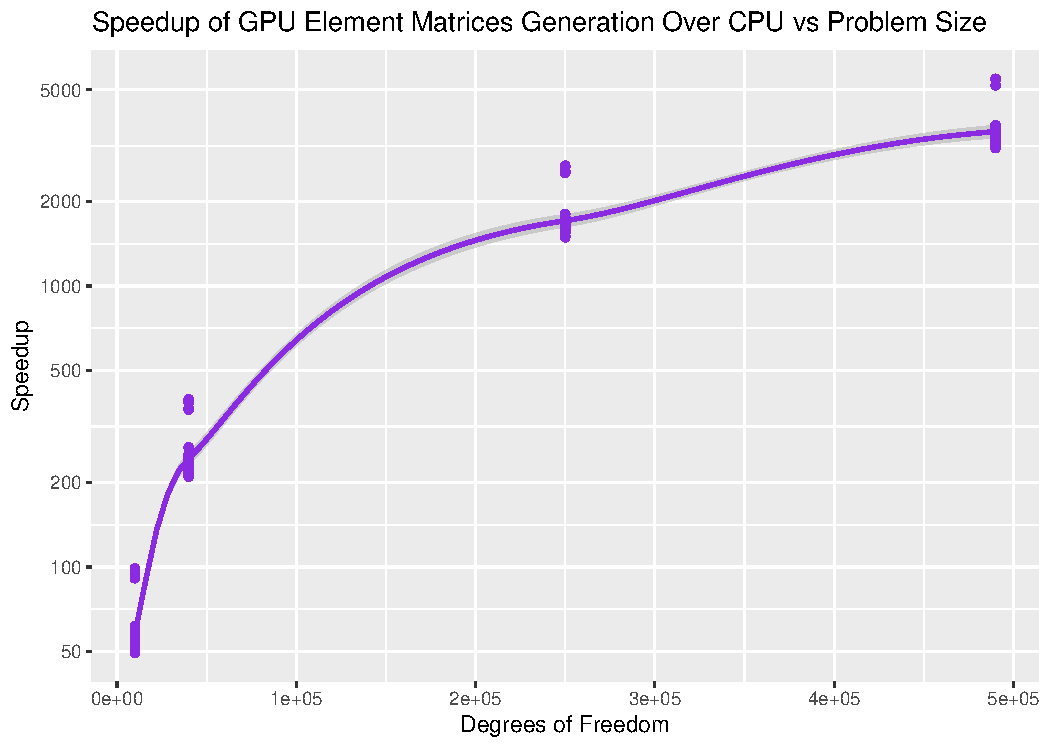
\includegraphics[width = \linewidth]{Plots/elem_mats_dev_cpu_speedup_vs_n}
		\caption{Speed-up over serial generation of element matrices versus problem size.}
		\label{fig:elems_n}
	\end{subfigure}\hfill
	\begin{subfigure}{0.48\linewidth}
		\centering
		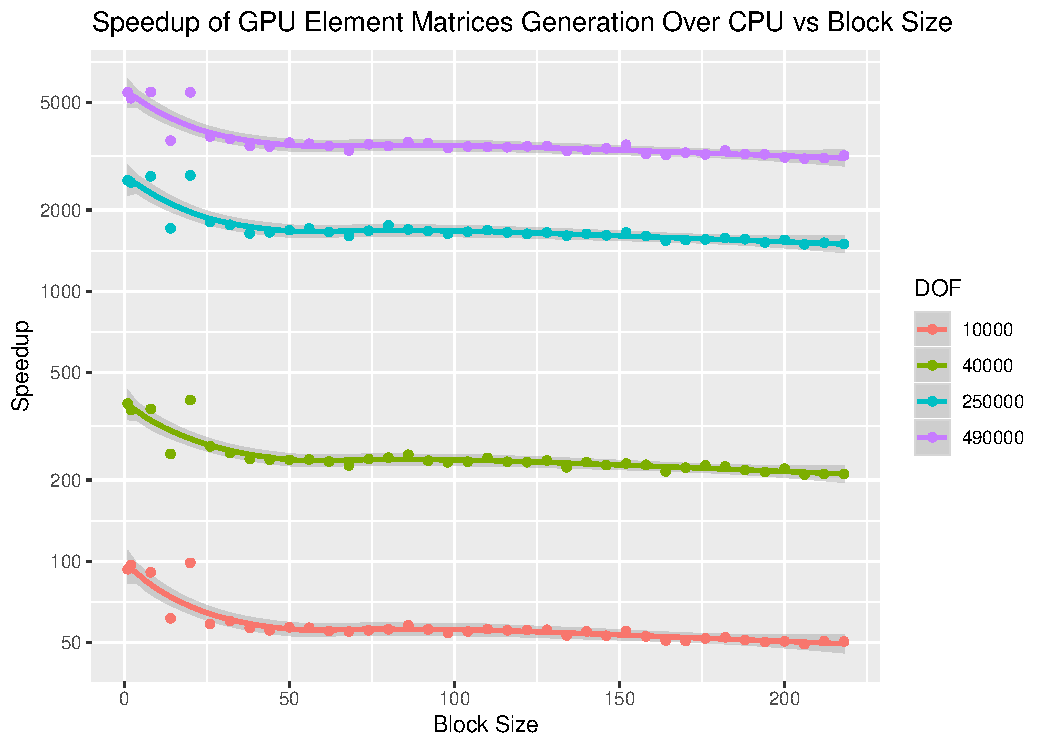
\includegraphics[width=\linewidth]{Plots/elem_mats_dev_cpu_speedup_vs_b}
		\caption{Speed-up over serial generation of element matrices versus blocks size.}
		\label{fig:elems_b}
	\end{subfigure}
	\caption{Speed-ups of GPU generation of element matrices and vectors over serial code against problem size ans block size.}
	\label{fig:elem_mats_gen}
\end{figure}

One of the two most relevant timings in this section is the generation of element matrices. As was discussed, there is a limited amount can be done about pre-existing linear solvers. However, there is a great deal of parallelism can be achieved when generating the element matrices and element vectors for the FEM. This is one of two of the the areas into which most of the thought regarding optimisation was put. All the considerations mentioned in Section~\ref{gpu_model} were taken into account here: optimising shared memory and registry usage, minimisation of thread divergence from warps, coalescing memory when at all possible et cetera.

Figure~\ref{fig:elem_mats_gen} shows the massive speed-ups seen over the CPU against both problem size and block size when the device function was measured. There is a massive logarithmic scaling as the degrees of freedom increases, reaching up to $5000\times$ faster than the serial code for the largest problem size tested. In terms of the comparison with block size, unlike in the pre-existing linear libraries, the choice of block size does matter here and is visible in Figure~\ref{fig:elems_b}, where there is a dip as block size increases - albeit it is not very clear what differences it makes after that. Figure~\ref{fig:elems_reconfig} demonstrates these same graphs but faceted by problem size. For considerations of shared memory, the CUDA devices tested in this paper, all come with a 1:3 ratio of thread registers to shared memory - specifically 16~Kb:48~Kb. There is quite a substantial amount of machinery needed for the FEM, resulting in a large amount of pointers to global and shared memory. Due to this, the thread registers end up overflowing. The conscious effort was made to use only a single shared memory pointer and avoid any unnecessary variables within device functions if at all possible. However, this can only help so much. Given that shared memory is quite large for the smaller block sizes, an added optimisation performed here was checking outside the kernel to deduce if there was shared memory spare, if there was, the memory was reconfigured to a 1:1 or 3:1 ratio to avoid and hedge against this overflow. The benefits are very clear in Figure~\ref{fig:elem_mats_gen}, observing more speed-up seen for all problem sizes. The overflow of thread registers is clear from the off as the drop-off seen in speed-up is observed from the smallest problem sizes.

Regarding thread divergence, it can be loosely seen that the speed-up appears to increase in and around multiples of 32. However, it isn't definitive for sure, and is almost certainly outweighed by the cost of memory transfer, to and from the thread registers overflowing into L2-cache.

\begin{figure}
	\centering
	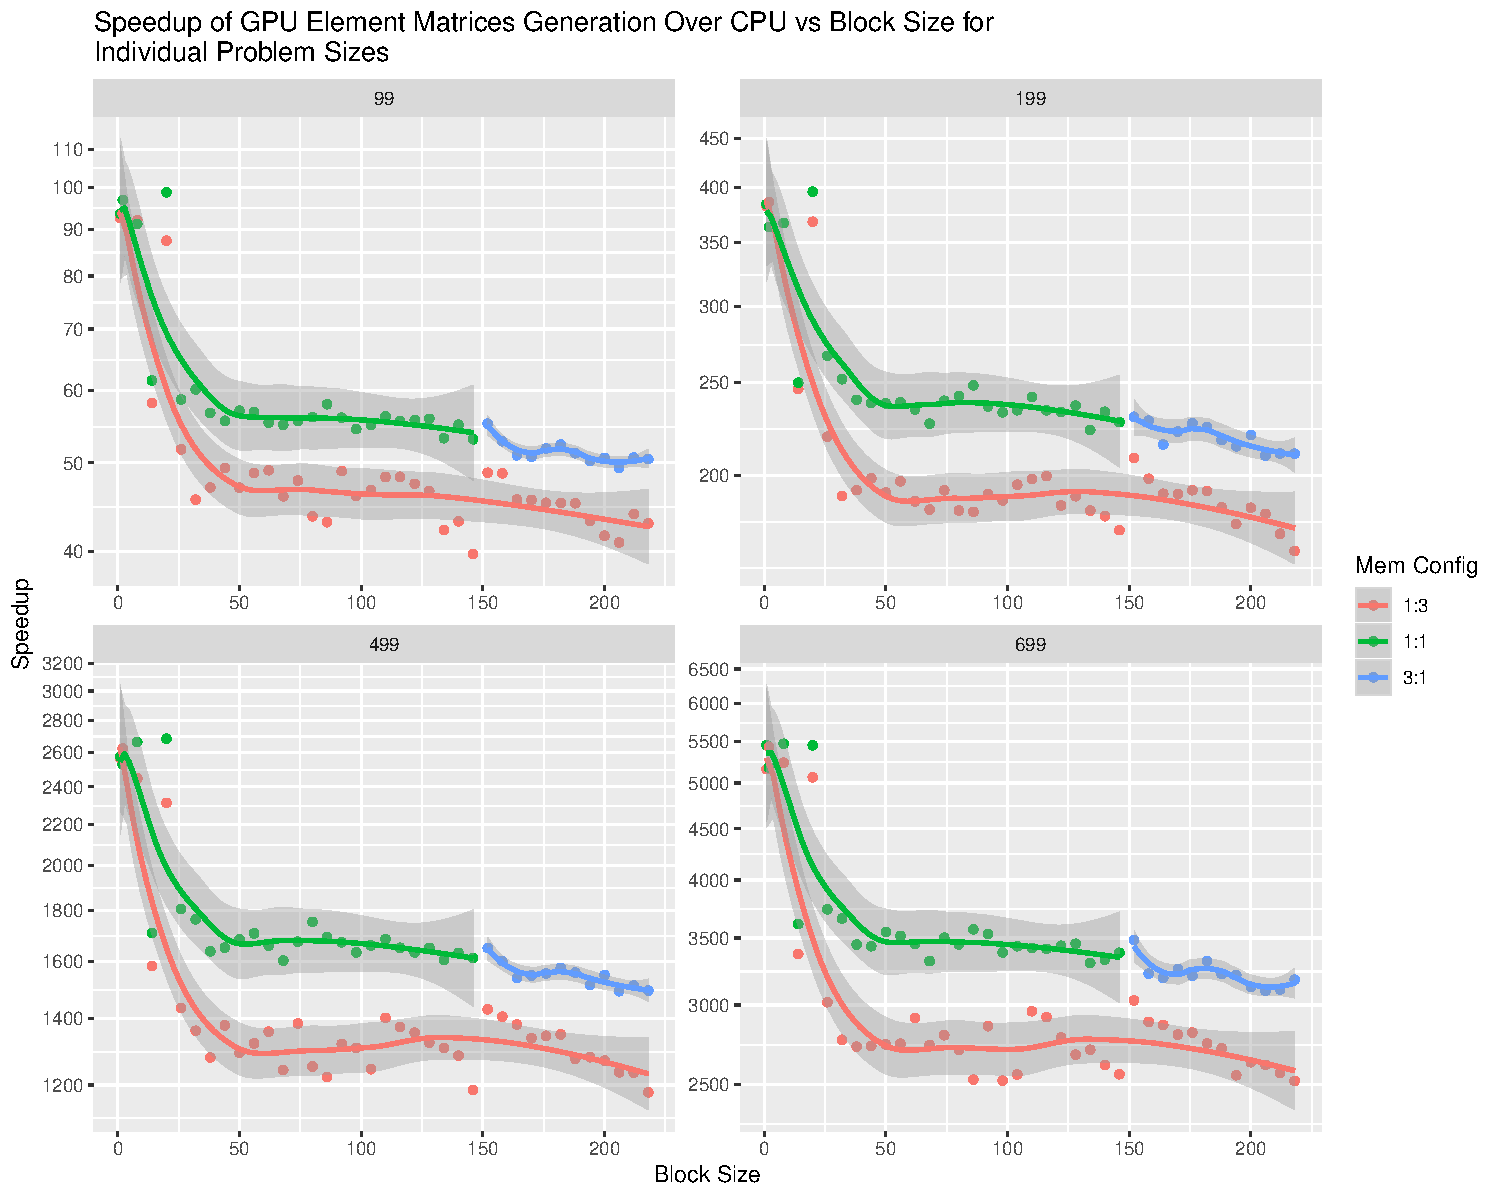
\includegraphics[width=0.9\linewidth]{Plots/elem_mats_dev_speedups_reconfig}
	\caption{Speed-up of GPU generation of element matrices over CPU versus block size for various problem sizes and memory configurations.}
	\label{fig:elems_reconfig}
\end{figure}

\subsubsection{Global Stiffness Matrix \& Stress Vector Assembly}

\begin{figure}
	\centering
	\begin{subfigure}{0.48\linewidth}
		\centering
		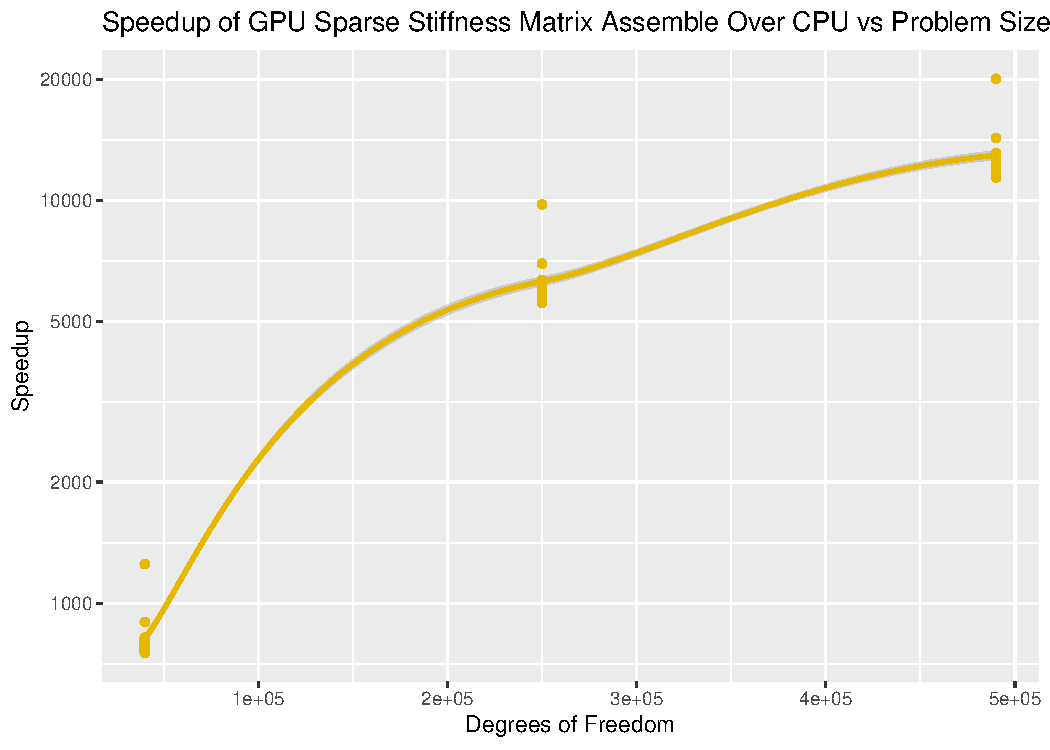
\includegraphics[width = \linewidth]{Plots/assem_dev_cpu_sparse_speedup_vs_n}
		\caption{Speed-up over serial assembly of CSR matrix.}
		\label{fig:assem_sparse_n}
	\end{subfigure}\hfill
	\begin{subfigure}{0.48\linewidth}
		\centering
		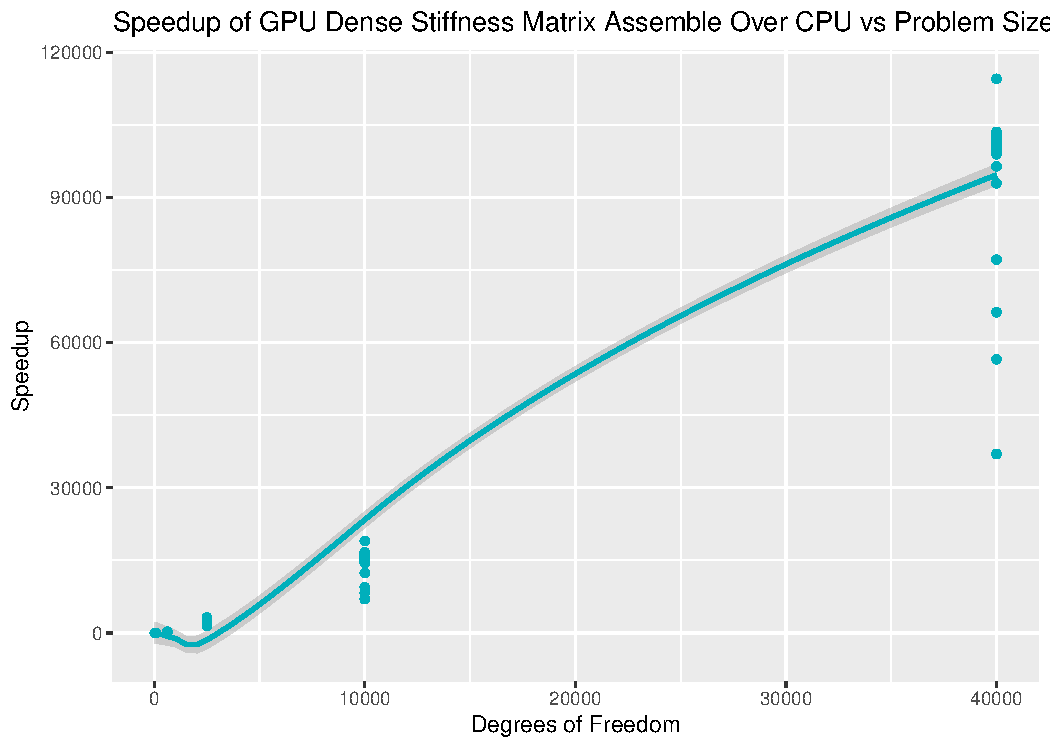
\includegraphics[width=\linewidth]{Plots/assem_dev_cpu_dense_speedup_vs_n}
		\caption{Speed-up over serial assembly of dense matrix.}
		\label{fig:assem_dense_n}
	\end{subfigure}
	\caption{Speed-ups of GPU generation of assembly of global stiffness matrix and stress vector over serial code against problem size for CSR and dense matrices.}
	\label{fig:assem_su_n}
\end{figure}

The assembly of the global stiffness matrix and stress vector are another important point of optimisation in this study, as it is another area which can provide huge amounts of parallelisation. Figure~\ref{fig:assem_su_n} shows the speed-ups seen for both sparse and dense variants of the device function, achieving even more impressive results than the element matrices generation. Both show massive speed-ups of $20,000\times$ and $100,000\times$, respectively. It might be an easy thought to assume that the sparse assembly would, in fact, be faster, but it turns out, to be slower than the dense assembly. Figure~\ref{fig:sparse_dense_assem} shows this fact. There are two contributing factors to this unexpected anomaly. The first being, there are far less variables, particularly pointers, needed in the dense assembly function and so the overflow of the, already-packed, registry memory is less of a factor. This can actually be seen in the initial spike, and quick drop off in speed-up seen in Figure~\ref{fig:sparse_dense_assem}, before the thread registers overflow in the sparse function. The second, main contributing factor to this, is the lack of coalescence and irregular memory access pattern of the CSR matrix. The algorithm requires jumping back and forward through three separate arrays to find the correct position in the matrix to perform an atomicAdd. This wouldn't particularly be an issue in the shared memory, but in global memory, this will provide quite a slow down. The dense assembly, however, is more rudimentary, and is also sequential accessing so does not suffer from these bottlenecks. So it then begs the question, which should have already an obvious answer, is the trade off for a sparse solver better than a dense assembly?

\begin{figure}
	\centering
	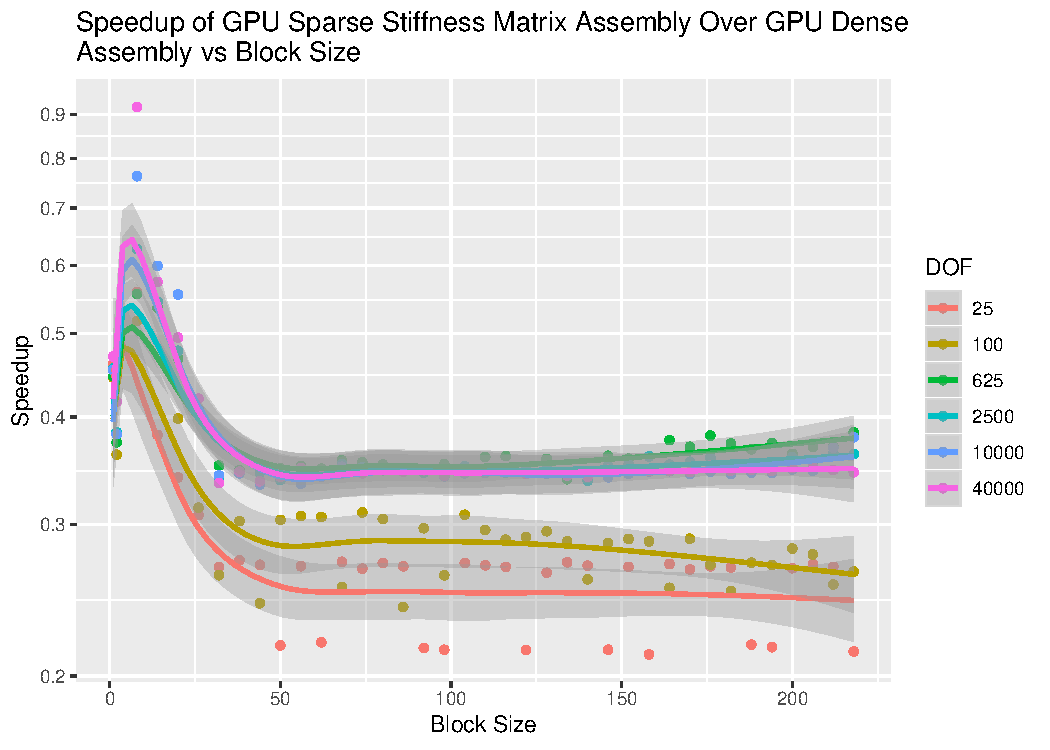
\includegraphics[width=0.55\linewidth]{Plots/assem_dev_gpu_sparse_dense_speedup_vs_b}
	\caption{Speed-ups of GPU sparse global stiffness matrix assembly over dense assembly versus block size.}
	\label{fig:sparse_dense_assem}
\end{figure}

Like in the element matrices, choice of block size does in fact matter - both for sparse and dense assembly. Figures~\ref{fig:assem_sparse_reconfig},~\ref{fig:assem_dense_reconfig} both show this. Like in the element matrices' device functions, there isn't a clear indication from the plots of thread divergence causing a large effect, but more so, oscillates slightly in and around multiples of 32 where the speed-ups increase. Again, also, reconfiguring the memory resulted in some positive results, barring overlaps in the smallest problem size. This could be down to the fact that all the threads in the block potentially not being used as the problem was not large enough.

\begin{figure}
	\centering
	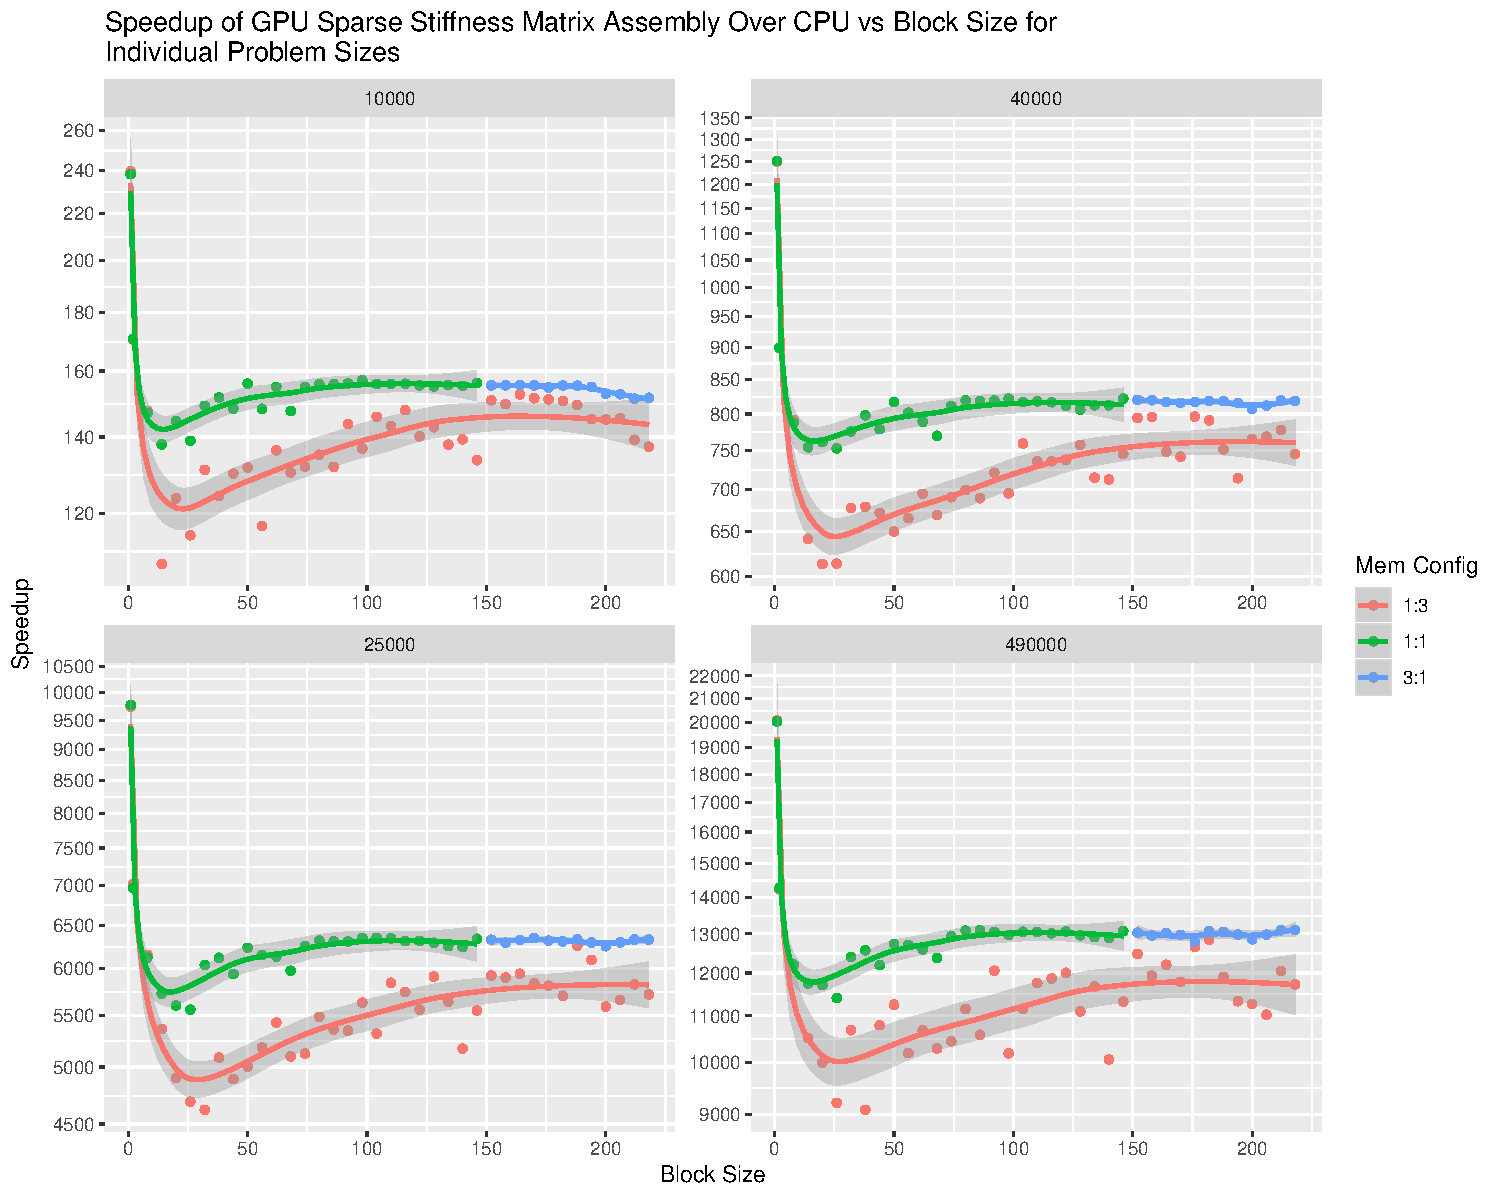
\includegraphics[width=0.9\linewidth]{Plots/assem_dev_sparse_speedups_reconfig}
	\caption{Speed-up of GPU assembly of sparse global stiffness matrix and stress vector over CPU versus block size for various problem sizes and memory configurations.}
	\label{fig:assem_sparse_reconfig}
\end{figure}

\begin{figure}
	\centering
	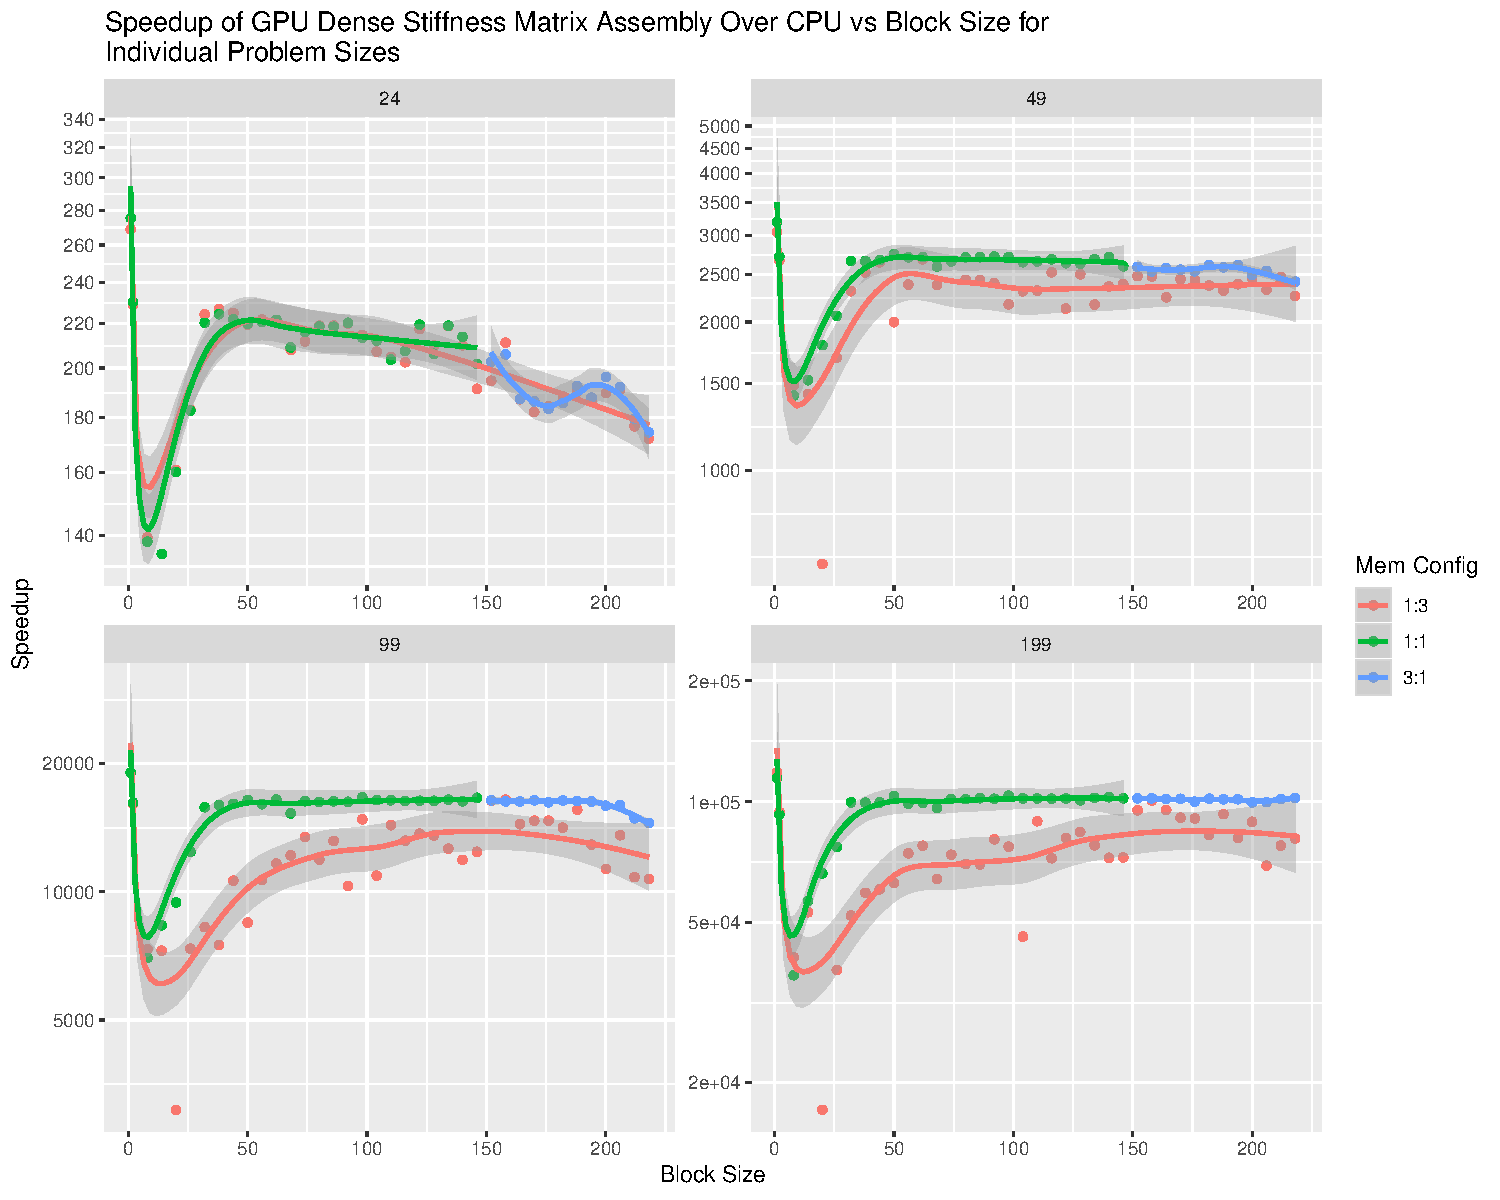
\includegraphics[width=0.9\linewidth]{Plots/assem_dev_dense_speedups_reconfig}
	\caption{Speed-up of GPU assembly of dense global stiffness matrix and stress vector over CPU versus block size for various problem sizes and memory configurations.}
	\label{fig:assem_dense_reconfig}
\end{figure}


\subsubsection{Main Kernel Total}

\begin{figure}
	\centering
	\begin{subfigure}{0.48\linewidth}
		\centering
		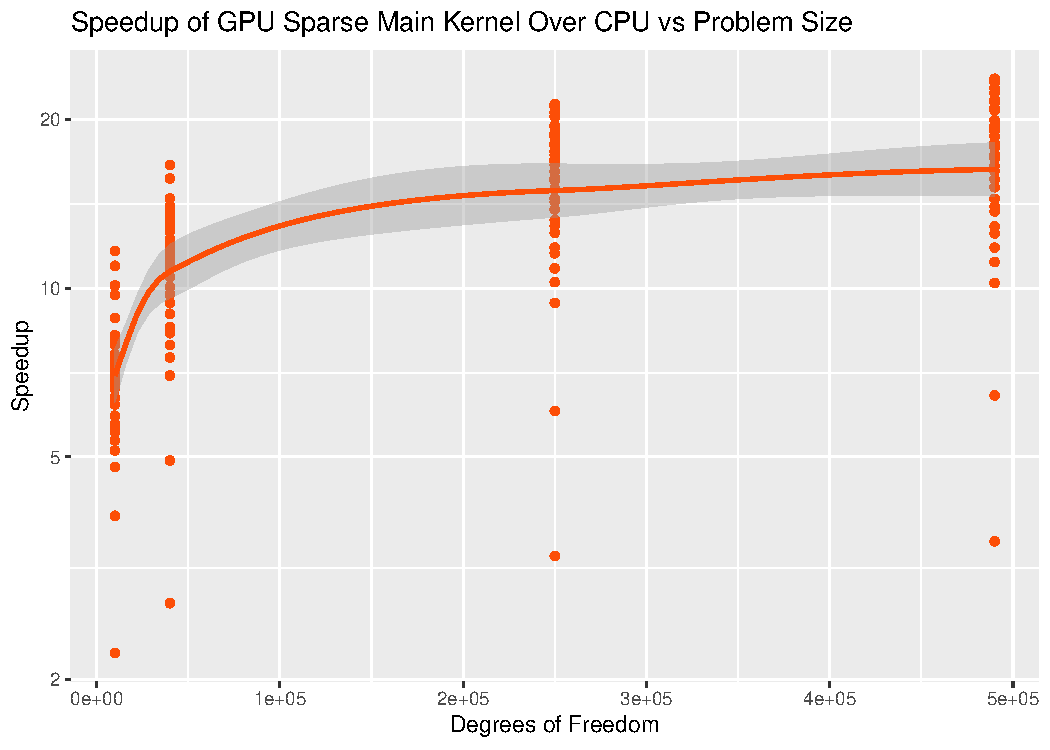
\includegraphics[width = \linewidth]{Plots/elems_p_assem_ker_cpu_sparse_speedup_vs_n}
		\caption{Speed-up of GPU main kernel over serial code for sparse case.}
		\label{fig:kern_sparse_n}
	\end{subfigure}\hfill
	\begin{subfigure}{0.48\linewidth}
		\centering
		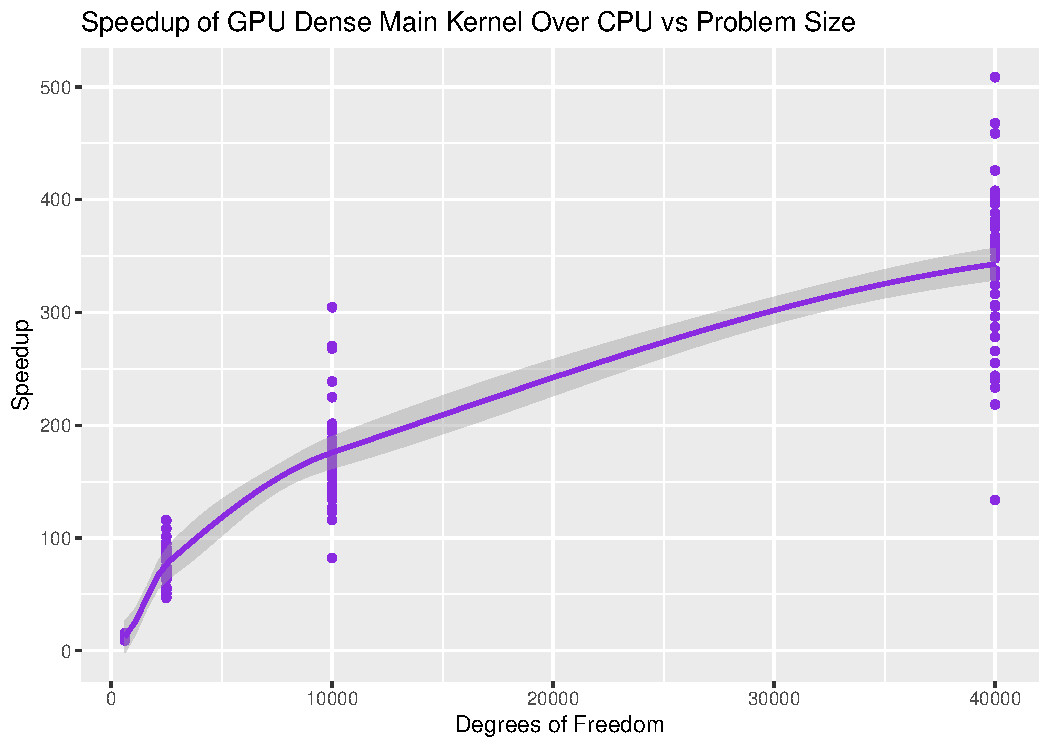
\includegraphics[width=\linewidth]{Plots/elems_p_assem_ker_cpu_dense_speedup_vs_n}
		\caption{Speed-up of GPU main kernel over serial code for sparse case.}
		\label{fig:kern_dense_n}
	\end{subfigure}
	\caption{Speed-ups of GPU main kernel over serial code against problem size for CSR and dense matrices.}
	\label{fig:kern_su_n}
\end{figure}

A downside to the timings for the two device functions is the lack of ability to use cudaEvents - which can only be used to time an kernel in its entirety. Instead, \texttt{clock64()} must to be utilised. This takes the clock ticks on each thread, which then must be written back to a global memory array, and then using cuBLAS, the max of this array calculated - giving the theoretical maximum time taken for the device function to finish. Unfortunately, in reality, that isn't how perfectly kernels and device functions run, as threads end up stalling while waiting for others and the kernel cannot complete until all the threads are finished. This is a bottleneck of CUDA programming and unavoidable. For example, when taking the cudaEvents time for the entire kernel, the irregular memory access pattern of writing these times into global memory must be taken into account as all the threads cannot finish the kernel until the entire array of clock cycles has been populated.

With that being said, for a more realistic speed-up time, the entire kernel was timed and these times are illustrated in Figures~\ref{fig:kern_sparse_n},~\ref{fig:kern_dense_n}. Even with the device timings being taken, the kernel still demonstrates faster execution times than in serial for both sparse and dense cases, reaching up to around $20\times$ and $300\times$, respectively. These times can be effectively taken as a minimum speed-up as removing the clock cycle evaluation will increase these even further.

Overall then, considering that the only part of the entire process that was attempted to be parallelised took up around 0.4\% of the entire computation time, the amount of speed-ups achieved in that small portion proved quite substantial.

\subsubsection{NVVP Profiling}

\begin{figure}
	\centering
	\begin{subfigure}{0.6\linewidth}
		\centering
		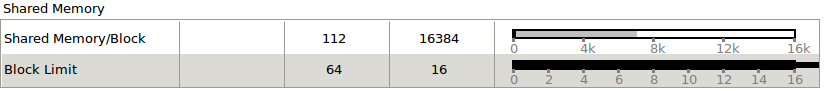
\includegraphics[width = \linewidth]{Figures/sparse_shared_1}
	\end{subfigure}\\
	\begin{subfigure}{0.6\linewidth}
		\centering
		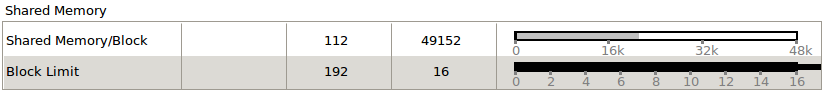
\includegraphics[width=\linewidth]{Figures/sparse_shared_M_1}
		\caption{Block size: 1}
	\end{subfigure}\\
	\begin{subfigure}{0.6\linewidth}
		\centering
		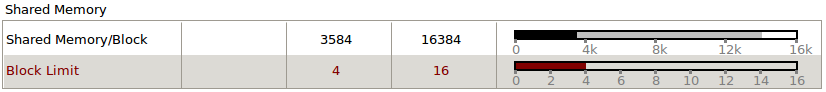
\includegraphics[width=\linewidth]{Figures/sparse_shared_32}
	\end{subfigure}
	\begin{subfigure}{0.6\linewidth}
		\centering
		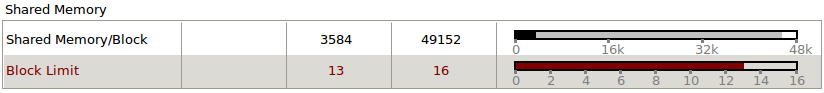
\includegraphics[width=\linewidth]{Figures/sparse_shared_M_32}
		\caption{Block size: 32}
	\end{subfigure}\\
	\begin{subfigure}{0.6\linewidth}
		\centering
		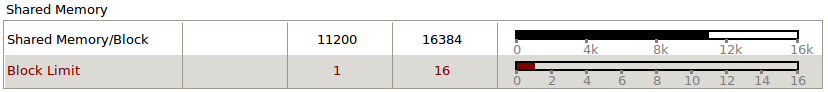
\includegraphics[width=\linewidth]{Figures/sparse_shared_100}
	\end{subfigure}\\
	\begin{subfigure}{0.6\linewidth}
		\centering
		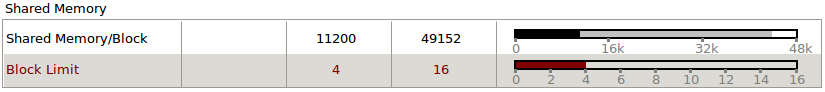
\includegraphics[width=\linewidth]{Figures/sparse_shared_M_100}
		\caption{Block size: 100}
	\end{subfigure}\\
	\begin{subfigure}{0.6\linewidth}
		\centering
		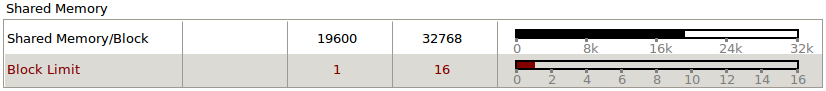
\includegraphics[width=\linewidth]{Figures/sparse_shared_175}
	\end{subfigure}\\
	\begin{subfigure}{0.6\linewidth}
		\centering
		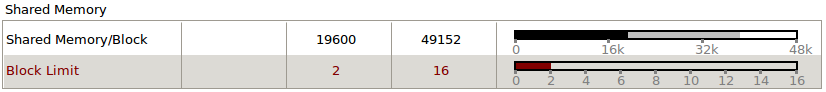
\includegraphics[width=\linewidth]{Figures/sparse_shared_M_175}
		\caption{Block size: 175}
	\end{subfigure}
	\caption{NVVP screenshots of shared memory occupation for four different block sizes, and with reconfiguration on and off.}
	\label{fig:sparse_mem_prof}
\end{figure}

For some extra profiling and analysis of the tool's performance, and deducing the levels of improvement seen by the various optimisations, Nvidia's Visual Profiler was used. Looking firstly at the memory usages, Figure~\ref{fig:sparse_mem_prof}, shows the shared memory occupation for four different block sizes, 1, 32, 100, and 175,  with memory reconfiguration both on and off. The smallest block size of 1 shows an obvious massive waste in available shared memory. This small block size does obviously mean more space for thread registers. However, without after reconfiguration it can be seen that the shared memory available goes from 49,152 bytes to 16,384 - gifting the registers the difference. It would make little to no sense to not do this when only 112 bytes per block are being used. As the block size increase, more optimal used of shared memory can be seen, stretching it towards its upper limits. For block size of 175 it is seen to switch to a 1:1 split since the shared memory required is actually above the 16~Kb available in the 3:1 split.

\begin{figure}
	\centering
	\begin{subfigure}{0.7\linewidth}
		\centering
		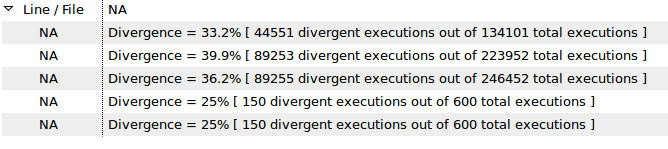
\includegraphics[width = \linewidth]{Figures/sparse_divergence_1}
		\caption{Block size: 1}
	\end{subfigure}\\
	\begin{subfigure}{0.7\linewidth}
		\centering
		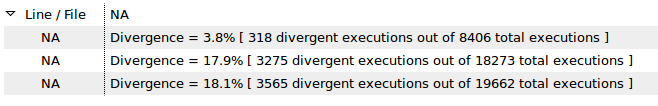
\includegraphics[width=\linewidth]{Figures/sparse_divergence_32}
		\caption{Block size: 32}
	\end{subfigure}\\
	\begin{subfigure}{0.7\linewidth}
		\centering
		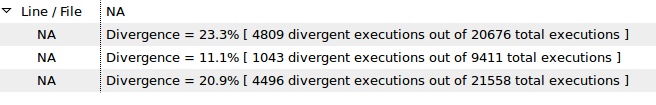
\includegraphics[width=\linewidth]{Figures/sparse_divergence_150}
		\caption{Block size: 150}
	\end{subfigure}\\
	\begin{subfigure}{0.7\linewidth}
		\centering
		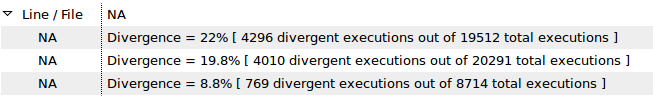
\includegraphics[width=\linewidth]{Figures/sparse_divergence_175}
		\caption{Block size: 175}
	\end{subfigure}
	\caption{NVVP screenshots of shared thread divergence for different block sizes.}
	\label{fig:sparse_diverge_prof}
\end{figure}

It was briefly touched upon that thread divergence is slightly visible from the plots earlier in this section, albeit only slightly. Figure~\ref{fig:sparse_diverge_prof} shows the thread divergence seen for three different block sizes 1, 32, 150 and 175 - all using the same problem size of course. It is evident here that multiples of 32 or even, the closer one is to multiples to 32, the less divergence is seen. The block size of 1 has the largest divergence with 150 and 175 more or less sharing 2\textsuperscript{nd} place. With that being said though, the difference is rather minimal and the gain is only in fact a few percent.

\begin{figure}
	\centering
	\includegraphics[width = 0.7\linewidth]{Figures/sparse_load}
	\caption{NVVP screenshot of load balance across SMs for main kernel of standard GPU approach.}
	\label{fig:sparse_load}
\end{figure}
A big factor in writing efficient parallel code is managing to balance the workload across the processing units as evenly as possibly. This seems entirely logical of course, as, if one thread has to do twice as much work as another, then the time taken will be slower than if they split 50:50. Figure~\ref{fig:sparse_load} shows the load balance across the 12 SMs on the GTX~780 card for the main kernel in the standard GPU approach. The results are quite even, with none of the SMs appearing to drop below 95\%.

\begin{figure}
	\centering
	\includegraphics[width = 0.55\linewidth]{Figures/sparse_instruction_latency}
	\caption{NVVP screenshot of latencies in main kernel of standard GPU approach.}
	\label{fig:sparse_latencies}
\end{figure}
The final thing looked at in NVVP was the instruction latency. Deducing the cause of your main latencies in your code can be a very good indication for why your CUDA code is not performing as optimally as you would have thought it to. Figure~\ref{fig:sparse_latencies} shows the latencies in the main kernel for the standard GPU approach. These are mainly dominated by memory latencies. The explanation of each of these terms are explained in Appendix (REFERENCE).

\subsection{FEMSES}

The FEMSES approach, also achieved some varying results in comparison to both the sparse and dense serial and standard GPU implementations. The main concern seen here, and also the main bottleneck was the slow rate of convergence. by comparison to the rates seen in Fernandez~\cite{femses}. This is address later in the section.

\subsubsection{Total Timings}

\begin{figure}
	\centering
	\begin{subfigure}{0.48\linewidth}
		\centering
		\includegraphics[width = \linewidth]{Plots/total_femses_cpu_sparse_speedup_vs_n}
		\caption{Total time speed-up of FEMSES over serial sparse solution.}
		\label{fig:tot_femses_sparse}
	\end{subfigure}\hfill
	\begin{subfigure}{0.48\linewidth}
		\centering
		\includegraphics[width=\linewidth]{Plots/total_femses_cpu_dense_speedup_vs_n}
		\caption{Total time speed-up of FEMSES over serial dense solution.}
		\label{fig:tot_femses_dense}
	\end{subfigure}\\
	\begin{subfigure}{0.48\linewidth}
		\centering
		\includegraphics[width=\linewidth]{Plots/total_femses_gpu_sparse_speedup_vs_n}
		\caption{Total time speed-up of FEMSES over GPU sparse solution.}
		\label{fig:tot_femses_gpu_sparse}
	\end{subfigure}\hfill
	\begin{subfigure}{0.48\linewidth}
		\centering
		\includegraphics[width=\linewidth]{Plots/total_femses_gpu_dense_speedup_vs_n}
		\caption{Total time speed-up of FEMSES over GPU dense solution.}
		\label{fig:tot_femses_gpu_dense}
	\end{subfigure}
	\caption{Speed-ups of total times over serial code and standard GPU code vs. problem size for FEMSES solution.}
	\label{fig:tot_femses}
\end{figure}

For the overall timings, the scaling trends were not wildly different to the ones seen in the other GPU implementation. Figure~\ref{fig:tot_femses} illustrates these speed-ups against both serial and alternate GPU approaches. For the sparse serial case, in Figure~\ref{fig:tot_femses_sparse}, the results are much the same as the other GPU approach where the parallel version is way outperformed by the serial due to Intel's DSS package. The scaling here even appears to decrease as problem size gets larger, after an initial increase. In Figure~\ref{fig:tot_femses_dense}, the story is much more positive, showing FEMSES to outperform the serial dense case at a logarithmic rate - reaching up to $10\times$ as fast. For comparison against the standard GPU approach, the sparse case in Figure~\ref{fig:tot_femses_gpu_sparse} shows quite poor scaling, initially outperforming the other approach, but as the solver kernel becomes more dominant as the problem size increase, there is an evident exponential decay in speed-up, to the point of being orders slower. The comparison to the GPU dense case in Figure~\ref{fig:tot_femses_gpu_dense} shows much the same results but begins to improve again as the problem size increases. This is more than likely down to the fact that the linear solver has less of an impact for the smaller problem sizes, and becomes more influential as the problem size increases. FEMSES, should, ideally scale better than the dense direct solver if its convergence achieved is at a short rate. Unfortunately, further problem sizes for the dense case couldn't be tested to check if this increase in speed-up is an anomaly due to restrictions on problem size in Intel's LAPACK library.

Contrary to what was seen in the other GPU FEM implementation, there is a lot more variation in results as block size changes for FEMSES. This is to be expected since out of the four kernels in the process, three of them are dependent on the block size - the exception being cuBLAS to evaluate the error at each iteration. Figures~\ref{fig:tot_femses_sparse_b},~\ref{fig:tot_femses_dense_b}, illustrate this massive amount of variability. This is far more erratic then the timings seen in the evaluation of the element matrices and assembly device functions in the previous section - even the confidence intervals seen by the shaded grey area of the loess regression are far larger. There isn't much inference can be made from the erraticity of these results, there definitely isn't any clear indication of thread divergence. One thing that can be deduced from them is there isn't any evidence of slowdown due to overflow of registers. It was difficult to deduce accurately what the cause of the scattered results is without proper per-kernel profiling and timings. However, it is discussed in the next section why this wasn't practical.

\begin{figure}
	\centering
	\includegraphics[width=0.9\linewidth]{Plots/total_femses_cpu_sparse_speedup_vs_b_facet}
	\caption{Speed-up of FEMSES total time over serial sparse case versus block size for various problem sizes.}
	\label{fig:tot_femses_sparse_b}
\end{figure}
\begin{figure}
	\centering
	\includegraphics[width = 0.9\linewidth]{Plots/total_femses_cpu_dense_speedup_vs_b_facet}
	\caption{Speed-up of FEMSES total time over serial dense case versus block size for various problem sizes.}
	\label{fig:tot_femses_dense_b}
\end{figure}

\subsubsection{Solver}

\begin{figure}
	\centering
	\begin{subfigure}{0.7\linewidth}
		\centering
		\includegraphics[width = \linewidth]{Figures/femses_prop_30}
		\caption{Degrees of Freedom size: 900}
	\end{subfigure}\\
	\begin{subfigure}{0.7\linewidth}
		\centering
		\includegraphics[width=\linewidth]{Figures/femses_prop_50}
		\caption{Degrees of Freedom size: 2,500}
	\end{subfigure}
	\begin{subfigure}{0.7\linewidth}
		\centering
		\includegraphics[width=\linewidth]{Figures/femses_prop_100}
		\caption{Degrees of Freedom size: 10,000}
	\end{subfigure}
	\caption{NVVP screenshots of proportion of computation time taken by each of the FEMSES kernels for different problem sizes.}
	\label{fig:femses_comp_prop}
\end{figure}

The FEMSES solver, like the linear system solvers in the previous sections, is the most dominant kernel in the process. It is, of course, divided up into three separate kernels for the GPU, the Jacobi iteration, the global solution assembly and the error evaluation. Unfortunately, to get any decent timings on these would involve adding cudaEvents to the code. These would be placed inside a while loop, which, while testing this in fact added up to 30\% extra computation time and so didn't actually prove a practical solution for profiling. Instead, the total solver time was timed for comparison with the other solutions, and the three individual kernels were profiled using Nvidia's Visual Profiler. Figure~\ref{fig:femses_comp_prop} shows the proportion of computation time taken by each of the kernels in the FEMSES approach individually. For small problem sizes, the error calculation is the most dominant. However, as this increases, the Jacobi solver becomes the dominating kernel. Figure~\ref{fig:solve_femses} shows the speed-ups over both serial and GPU solutions for the FEMSES solver. Again, due to the dominance of the solver step of the entire process, it has almost replicated the results seen in Figure~\ref{fig:tot_femses}. Unfortunately, the performance over the sparse cases leave a lot to be desired, but again, this is going to be primarily due to the unforeseen slower rate of convergence than anticipated.

\begin{figure}
	\centering
	\begin{subfigure}{0.48\linewidth}
		\centering
		\includegraphics[width = \linewidth]{Plots/solve_femses_sparse_cpu_speedup_vs_n}
		\caption{FEMSES solver speed-up over Intel's MKL DSS.}
		\label{fig:solve_femses_sparse}
	\end{subfigure}\hfill
	\begin{subfigure}{0.48\linewidth}
		\centering
		\includegraphics[width=\linewidth]{Plots/solve_femses_dense_cpu_speedup_vs_n}
		\caption{FEMSES solver speed-up over Intel's MKL LAPACKE dense solver.}
		\label{fig:solve_femses_dense}
	\end{subfigure}\\
	\begin{subfigure}{0.48\linewidth}
		\centering
		\includegraphics[width=\linewidth]{Plots/solve_femses_sparse_gpu_speedup_vs_n}
		\caption{FEMSES solver speed-up over cuSOLVER's sparse solver.}
		\label{fig:solve_femses_gpu_sparse}
	\end{subfigure}\hfill
	\begin{subfigure}{0.48\linewidth}
		\centering
		\includegraphics[width=\linewidth]{Plots/solve_femses_dense_gpu_speedup_vs_n}
		\caption{FEMSES solver speed-up over cuSOLVER's dense solver.}
		\label{fig:solve_femses_gpu_dense}
	\end{subfigure}
	\caption{Speed-ups of FEMSES solver times over Intel's MKL and cuSOLVER versus problem size.}
	\label{fig:solve_femses}
\end{figure}

\subsubsection{Allocations \& Transfers}

\begin{figure}
	\centering
	\includegraphics[width=0.48\linewidth]{Plots/alloc_femses_vs_n}
	\caption{Allocation time for FEMSES versus problem size}
	\label{fig:alloc_femses}
\end{figure}
The allocation time for the FEMSES approach is shown in Figure~\ref{fig:alloc_femses}. It demonstrates an expected linear scaling (barring one outlier within the 95\% confidence allowance). The allocation here involves, as before, the five mesh arrays, as well as an array containing all the element matrices and the element vectors, as well as the weightings. All of these arrays have linear scaling and there is no dense global stiffness matrix so the linear scaling was to be expected. Figure~\ref{fig:alloc_femses_su} shows the speed-up over the other two GPU implementations. FEMSES manages to take roughly the same amount of allocation time as the sparse approach at small problem sizes, but as this grows, the scaling of the CSR matrix scales better than the array of all the element matrices and element vectors along with the weighting vector - hence the evident decline as the degrees of freedom grows. The dense case, on the other hand, scales far worse than FEMSES - to be expected since there is no dense stiffness matrix allocated. There is a nice logarithmic scaling, reaching up to $7.5\times$ speed-up.

\begin{figure}
	\centering
	\begin{subfigure}{0.48\linewidth}
		\centering
		\includegraphics[width =\linewidth]{Plots/alloc_femses_sparse_speedup_vs_n}
		\caption{Speed-up over sparse case.}
		\label{fig:alloc_femses_sparse}
	\end{subfigure}\hfill
	\begin{subfigure}{0.48\linewidth}
		\centering
		\includegraphics[width=\linewidth]{Plots/alloc_femses_dense_speedup_vs_n}
		\caption{Speed-up over dense case.}
		\label{fig:alloc_femses_dense}
	\end{subfigure}
	\caption{Speed-ups of FEMSES allocation time over GPU sparse \& dense solutions.}
	\label{fig:alloc_femses_su}
\end{figure}

There was no transfer times taken for FEMSES as the amount of data required to be transferred is identical to that of the GPU dense approach - the mesh and solution vector.
  
\subsubsection{Convergence}

\begin{figure}
	\centering
	\includegraphics[width=0.58\linewidth]{Plots/iters_v_n}
	\caption{Number of iterations for convergence of the FEMSES approach versus problem size with abline of linear scale for reference.}
	\label{fig:converg}
\end{figure}
The poor rate of convergence was the main concern regarding the FEMSES implementation. Figure~\ref{fig:converg} illustrates the convergence as problem size increases and shows the super-linear rate which it achieves. When investigating why these results may be happening, one thing which was noticed, as the errors got smaller, they often reached orders of $10^{-5}$ and $10^{-6}$ and then proceeded to oscillate in and around these values, never reaching convergence within maximum iterations. The error then had to be truncated to $10^{-4}$ to avoid this. An inclination here was that the paper may have been using double precision and this was down to accuracy lost from utilising single precision values instead. This was tested and the results proved equal. The current proposal as to the reasoning for these unexpected results is in Fernandez~\cite{femses}, the PDE used is a rectangular pipe, with non-homogeneous Dirichlet conditions on the outer boundaries and homogeneous Neumann on the bore hole, thus causing propagation from four directions. In the example in Section~\ref{problem}, the rectangular mesh has homogeneous Neumann conditions on the upper and lower edges and non-homogeneous Dirichlet conditions on the left and right boundary, therefore propagation will occur in only two directions, from left and right inwards. This theory has yet to be tested but would be an interesting result to deduce if this is indeed the root cause of the sub-par performance of FEMSES. 

\subsubsection{NVVP Profiling}

\begin{figure}
	\centering
	\includegraphics[width = 0.7\linewidth]{Figures/femses_divergence}
	\caption{NVVP screenshots showing the lack of thread divergence for the all FEMSES kernels.}
	\label{fig:femses_diverge_prof}
\end{figure}

Regarding warps, it was stated in this section that there really wasn't any clear indication of the presence of thread divergence in the FEMSES code. This was profiled with NVVP and Figure~\ref{fig:femses_diverge_prof} shows the output from this. It was tested for various block sizes, multiples of 32 and not, and for all contributing kernels, and in all cases there was no resulting thread divergence indicated by the profiler. This would explain to a certain extent why the erratic graphs didn't show any pattern.

\begin{figure}
	\centering
	\begin{subfigure}{0.7\linewidth}
		\centering
		\includegraphics[width = \linewidth]{Figures/femses_jacobi_load}
		\caption{Load balancing for local solutions kernel.}
	\end{subfigure}\\
	\begin{subfigure}{0.7\linewidth}
		\centering
		\includegraphics[width=\linewidth]{Figures/femses_glob_load}
		\caption{Load balancing for global solutions kernel.}
	\end{subfigure}
	\caption{NVVP screenshots of shared load balance across SMs for two of the main kernels in the FEMSES approach.}
	\label{fig:femses_load}
\end{figure}

For load balancing the code, Figure~\ref{fig:femses_load} shows the distribution of workload across the SMs for two of the kernels written for FEMSES - cuBLAS nrm2 was ignored as it wasn't the job of this report to optimise it and the element matrices kernel as it was profiled in the standard GPU approach. Both kernels are quite load balanced, though the Jacobi iteration kernel does show a certain degree of lacking in compute utilisation.

\begin{figure}
	\centering
	\begin{subfigure}{0.43\linewidth}
		\centering
		\includegraphics[width = \linewidth]{Figures/femses_jacobi_instruction_latency}
		\caption{Latencies for Jacobi iteration kernel.}
	\end{subfigure}\hfill
	\begin{subfigure}{0.48\linewidth}
		\centering
		\includegraphics[width=\linewidth]{Figures/femses_glob_instruction_latency}
		\caption{Latencies for global solutions kernel.}
	\end{subfigure}
	\caption{NVVP screenshots of computation latencies for two of the main kernels in the FEMSES approach.}
	\label{fig:femses_latencies}
\end{figure}

Lastly, the stalling profiling. Figure~\ref{fig:femses_latencies} illustrates the latency reasons for both of the main kernels in the FEMSES approach - again, excluding the element matrices and error kernels. These latencies are quite evenly distributed across various reasons. Again, these are all explained in Appendix (REFERENCE).

\subsection{Comparison of GPU Architectures}

Two different GPUs were used in testing for this paper. All the results seen in the previous section are all taken from the Tesla~K40. The RTX~2080 Super was installed recently and due to time constraints didn't complete an entire test suite, but rather only completed tests for a single block size. The problem size was also limited to smaller values than the Tesla due to memory limitations of the RTX~2080 having smaller DRAM. In this section, the performance of the RTX~2080 Super is compared against the older Tesla~K40.

\subsubsection{Total Timings \& Solvers}

\begin{figure}
	\centering
	\begin{subfigure}{0.48\linewidth}
		\centering
		\includegraphics[width = \linewidth]{Plots/total_sparse_rtx_speedup_vs_n}
		\caption{Total time speed-up of RTX~2080 over Tesla~K40 for sparse solution.}
		\label{fig:total_rtx_sparse}
	\end{subfigure}\hfill
	\begin{subfigure}{0.48\linewidth}
		\centering
		\includegraphics[width=\linewidth]{Plots/total_dense_rtx_speedup_vs_n}
		\caption{Total time speed-up of RTX~2080 over Tesla~K40 for dense solution.}
		\label{fig:total_rtx_dense}
	\end{subfigure}\\
	\begin{subfigure}{0.48\linewidth}
		\centering
		\includegraphics[width=\linewidth]{Plots/total_femses_rtx_speedup_vs_n}
		\caption{Total time speed-up of RTX~2080 over Tesla~K40 for FEMSES.}
		\label{fig:total_rtx_femses}
	\end{subfigure}
	\caption{Speed-ups RTX~2080 over Tesla~K40 of total times versus problem size for three main approaches.}
	\label{fig:total_rtx}
\end{figure}

The total times appeared to achieve mostly more positive results on the RTX~2080 than on the Tesla. The speed-ups over the Tesla versus problem size are illustrated in Figure~\ref{fig:total_rtx}. The sparse case demonstrates a nice stable speed-up of around $2\times$, while the dense case appears to experience some form of linear or possibly slightly logarithmic scaling, to a higher degree of up to $4\times$, roughly. FEMSES on the other hand, actually appeared to perform worse on the newer architecture. It does experience a positive scaling trend but never appears to actually outperform the older card.

\begin{figure}
	\centering
	\begin{subfigure}{0.48\linewidth}
		\centering
		\includegraphics[width = \linewidth]{Plots/solve_sparse_rtx_speedup_vs_n}
		\caption{Solver time speed-up of RTX~2080 over Tesla~K40 for sparse solution.}
		\label{fig:solve_rtx_sparse}
	\end{subfigure}\hfill
	\begin{subfigure}{0.48\linewidth}
		\centering
		\includegraphics[width=\linewidth]{Plots/solve_dense_rtx_speedup_vs_n}
		\caption{Solver time speed-up of RTX~2080 over Tesla~K40 for dense solution.}
		\label{fig:solve_rtx_dense}
	\end{subfigure}\\
	\begin{subfigure}{0.48\linewidth}
		\centering
		\includegraphics[width=\linewidth]{Plots/solve_femses_rtx_speedup_vs_n}
		\caption{Solver time speed-up of RTX~2080 over Tesla~K40 for FEMSES.}
		\label{fig:solve_rtx_femses}
	\end{subfigure}
	\caption{Speed-ups RTX~2080 over Tesla~K40 of solver times versus problem size for three main approaches.}
	\label{fig:solve_rtx}
\end{figure}

In Figure~\ref{fig:solve_rtx}, the speed-ups are shown against problem size for the solver kernel in the process. Again, just like the results seen on the Tesla, the solver is evidently the dominant kernel in the method and the resulting graphs are near identical. These results do somewhat explain the poorer performance in the FEMSES approach than the other two methods. It is largely possibly that the cuSOLVER libraries have been optimised to work well with the newer Nvidia architectures and take advantage of whichever technologies these may bring. However, the FEMSES approach has most of its code purpose written for this report and coded almost entirely on the Tesla and so, expectedly, performs quite well on this by comparison.

\subsubsection{Generation of Element Matrices \& Assembly of Global System}

\begin{figure}
	\centering
	\begin{subfigure}{0.48\linewidth}
		\centering
		\includegraphics[width = \linewidth]{Plots/elems_rtx_speedup_vs_n}
		\caption{Generation of element matrices time speed-up of RTX~2080 over Tesla~K40.}
		\label{fig:elems_rtx}
	\end{subfigure}\hfill
	\begin{subfigure}{0.48\linewidth}
		\centering
		\includegraphics[width=\linewidth]{Plots/assem_sparse_rtx_speedup_vs_n}
		\caption{Assembly of global system time speed-up of RTX~2080 over Tesla~K40 for sparse solution.}
		\label{fig:assem_rtx_sparse}
	\end{subfigure}\\
	\begin{subfigure}{0.48\linewidth}
		\centering
		\includegraphics[width=\linewidth]{Plots/assem_dense_rtx_speedup_vs_n}
		\caption{Assembly of global system time speed-up of RTX~2080 over Tesla~K40 for dense solution.}
		\label{fig:assem_rtx_dense}
	\end{subfigure}
	\caption{Speed-ups RTX~2080 over Tesla~K40 of different kernel times versus problem size for three main approaches.}
	\label{fig:kerns_rtx}
\end{figure}

The speed-ups of time taken for the generation of element matrices and the assembly of both sparse and dense global linear systems are shown in Figure~\ref{fig:kerns}. Both the generation of the element matrices and the assembly of the sparse solution achieve relatively stable speed-ups of about $5\times$.  Positive results in both instances. The dense assembly speed-up  is a little harder to make inferences from. Given that the sample size for these tests is much smaller (evident from the large confidence intervals in the plots), there appears to be an outlier for problem sizes of 1000. Besides this, although the trend is negative, the dense assembly also showed positive speed-ups for various the number of unknowns tested.

\subsubsection{Allocations \& Transfers}

\begin{figure}
	\centering
	\begin{subfigure}{0.48\linewidth}
		\centering
		\includegraphics[width = \linewidth]{Plots/alloc_sparse_rtx_speedup_vs_n}
		\caption{Allocation time speed-up of RTX~2080 over Tesla~K40 for sparse solution.}
		\label{fig:alloc_rtx_sparse}
	\end{subfigure}\hfill
	\begin{subfigure}{0.48\linewidth}
		\centering
		\includegraphics[width=\linewidth]{Plots/alloc_dense_rtx_speedup_vs_n}
		\caption{Allocation time speed-up of RTX~2080 over Tesla~K40 for dense solution.}
		\label{fig:alloc_rtx_dense}
	\end{subfigure}\\
	\begin{subfigure}{0.48\linewidth}
		\centering
		\includegraphics[width=\linewidth]{Plots/alloc_femses_rtx_speedup_vs_n}
		\caption{Allocation time speed-up of RTX~2080 over Tesla~K40 for FEMSES.}
		\label{fig:alloc_rtx_femses}
	\end{subfigure}
	\caption{Speed-ups RTX~2080 over Tesla~K40 of allocation times versus problem size for three main approaches.}
	\label{fig:alloc_rtx}
\end{figure}

Figure~\ref{fig:alloc_rtx} shows the speed-ups in allocation time for the three different approaches. The speed-up see for allocating the sparse matrices, again shows a nice stable speed-up of about $2\times$ as fast as the old card. The dense and FEMSES case both have more unusual trends. The dense case, ignoring a massive spike outlier, appears to also be quite stable at $1.4\times$, but there is an outlier nonetheless. For the FEMSES case the graph demonstrates what appears to be logarithmic scaling at a glance. Difficult to deduce why this is the case other than on the bad side of variance with clock speeds on the card while testing.

\begin{figure}
	\centering
	\begin{subfigure}{0.48\linewidth}
		\centering
		\includegraphics[width = \linewidth]{Plots/transfer_sparse_rtx_speedup_vs_n}
		\caption{Transfer time speed-up of RTX~2080 over Tesla~K40 for sparse solution.}
		\label{fig:transf_rtx_sparse}
	\end{subfigure}\hfill
	\begin{subfigure}{0.48\linewidth}
		\centering
		\includegraphics[width=\linewidth]{Plots/transfer_dense_rtx_speedup_vs_n}
		\caption{Transfer time speed-up of RTX~2080 over Tesla~K40 for dense solution/FEMSES.}
		\label{fig:transf_rtx_dense}
	\end{subfigure}
	\caption{Speed-ups RTX~2080 over Tesla~K40 of transfer times versus problem size for sparse and dense solutions.}
	\label{fig:trasnf_rtx}
\end{figure}

Again, similar to the allocation times, the transfer times in Figure~\ref{fig:trasnf_rtx}, appeared quite stable for the CSR cases and then quite erratic for the dense case. This is also an unusual result and presumably down to the same issues seen in the other cases. This would make sense as the problem size causing the spikes appears to be the same for all the outliers. Besides this, however, again positive speed-ups are obeserved.

All considered then, it's clear that the newer architecture, overall, outperformed the Tesla. It would be interesting to investigate further the potential speed-ups that could be achieved with this new card given more time for testing.
